\subsection{Esquema general}
El hardware principal de Solar Link se compone de 3 plaquetas principales:

\begin{itemize}
    \item \textbf{Motherboard:} Es donde se encuentra el microcontrolador principal ESP32. Esto implica que es el núcleo del proyecto, y tiene que poder transmitir y recibir información hacia y desde todo el resto de módulos.
    \item \textbf{Medidor de corriente:} Este módulo posee los sensores de corriente no invasivos. A través de estos, podemos medir independientemente la corriente que circula por cada una de las dos líneas que utilizamos.
    \item \textbf{Módulo de conmutación:} Se encarga de switchear entre la línea del proveedor eléctrico y la línea de energía solar.
\end{itemize}

Este hardware se presenta en un tablero eléctrico, el cual reduce al mínimo las interferencias por ruido eléctrico, y permite que el sistema quede protegido frente al uso diario.\\

Este tablero también posee, a modo de prototipo, dos entradas de línea, una se conecta a la red eléctrica convencional, y otra a la línea de energía solar, dos salidas independientes, las cuales son dos zapatillas representando la línea de una casa, y una ficha de comunicación, la cual se conecta al cargador MPPT para recibir información sobre la carga de la batería. Además, posee una antena WIFI para la ESP32.\\

El sistema es alimentado por dos transformadores 220V-9+9V, uno para la motherboard y el medidor de corriente, y otro exclusivo para el módulo de conmutación. Fue necesario el uso de un transformador exclusivo para esta última placa debido al alto consumo que representan los relés.\\

La señal entrante se rectifica con el circuito de la figura \ref{fig:Fuente 12v}, el cual, utilizando el punto medio de los transformadores, rectifica la señal de 9V de alterna, convirtiéndola en una de aproximadamente 12V.\\

\begin{figure}[H]
    \centering
    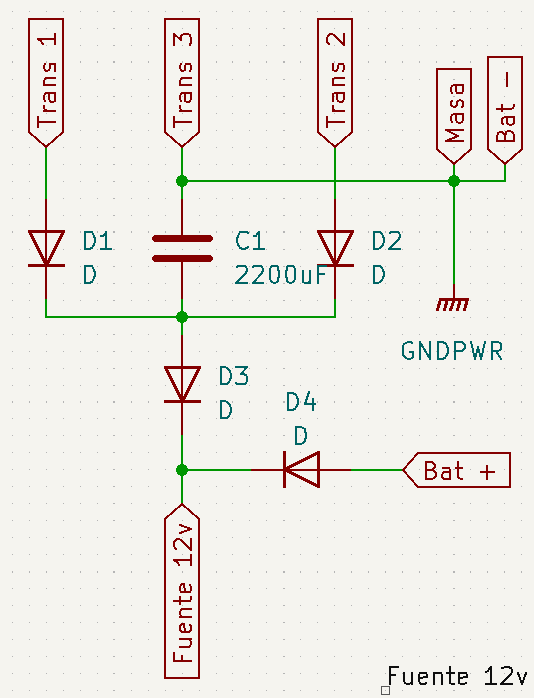
\includegraphics[width=0.7\linewidth]{hardware/Screenshot_10.png}
    \caption{Fuente 12V de Solar Link para los relés.}
    \label{fig:Fuente 12v}
\end{figure}

Por otra parte, a este circuito también entran los 12V de la batería. Gracias a los diodos en el circuito, la señal de salida resultará de la fuente con mayor potencial. De esta manera, frente a un corte de suministro eléctrico, el sistema seguirá funcionando con la energía de la batería.\\

Para mostrar la información medida, utilizamos un LCD de 20x04, colocado en la tapa del tablero. De esta manera, se pueden visualizar estos valores a simple vista sin tener que acceder a la aplicación o necesidad de abrir el tablero mismo.\\

\subsection{Motherboard}

\subsubsection{Sistema embebido}

El núcleo de nuestro proyecto es el microcontrolador ESP32. Es una placa de desarrollo que y trabaja con el microprocesador Tensilica Xtensa LX6 de 32 bits y 2 núcleos. Además, cuenta con periféricos como UART, I2C, ADC, Wi-Fi, Bluetooth, entre otros.\\

\begin{figure}[H]
    \centering
    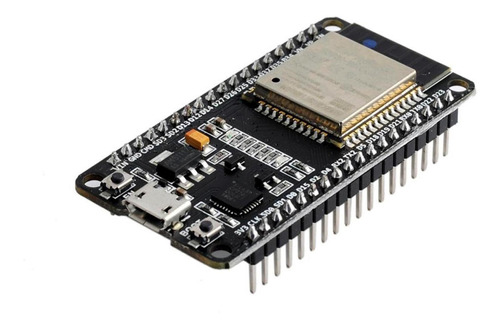
\includegraphics[width=0.75\linewidth]{hardware/ESP32.jpg}
    \caption{Placa de desarrollo ESP32 Devkit V 1.0}
    \label{fig:ESP32}
\end{figure}

Esta placa cuenta con 2 ADC internos de 12 bits de resolución, los cuales pueden trabajar hasta con 15 entradas diferentes. Se realizan únicamente 2 mediciones con ADCs, voltaje de batería y de línea, por lo tanto se asigna cada una a un ADC diferente, optimizando el uso de ambos para lograr mejores mediciones.\\

El periférico de comunicación I2C se utiliza para comunicarse con el ADC externo ADS1115 (figura \ref{fig:ads1115}), y para el LCD de 20x04. Por otra parte, el periférico de comunicación UART es utilizado para recibir información de la Raspberry Pi Pico del cargador MPPT.\\

El módulo Wi-Fi es utilizado para transmitir toda la información recabada hacia la aplicación, la cual se encarga de organizarla para que se pueda visualizar de una manera agradable y entendible.\\

Se aprovechan los dos núcleos del microprocesador para realizar todas las mediciones y comunicaciones en uno, y en el otro enviar la información por medio de Wi-Fi. Esto, en caso de un fallo en este módulo, no se congele el resto de instrucciones, además de poder realizarlas con mayor velocidad por estar distribuidas.\\

\subsubsection{Mediciones realizadas}

En la motherboard de Solar Link, se realizan 3 mediciones independientes: voltaje de línea, voltaje de batería, y cruce por cero.\\

Para medir el voltaje de línea, se utiliza el circuito de la figura \ref{fig:Vlinea}. Este cuenta con un rectificador de media onda y un capacitor conectados a la salida del tranformador, resultando en un voltaje de continua proporcional al voltaje de la línea de la casa. Como el valor de esa señal de continua es muy grande, se utiliza un divisor resistivo que disminuye la tensión en una escala donde el ADC lo puede leer sin problema.\\

\begin{figure}[H]
    \centering
    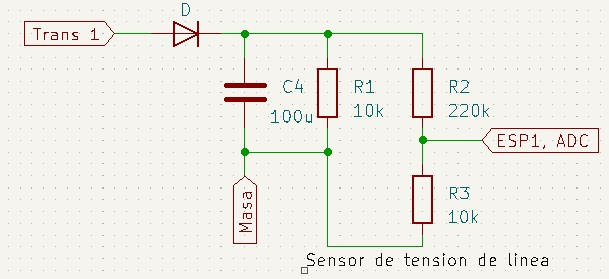
\includegraphics[width=0.9\linewidth]{hardware/Screenshot_14.jpg}
    \caption{Circuito de medición de tensión de línea.}
    \label{fig:Vlinea}
\end{figure}

El voltaje de la batería, al ya ser una señal de continua, simplemente se utiliza un divisor de tensión para medirlo (figura \ref{fig:Vbat}). Si bien este valor tambien lo lee y comparte el cargador, se mide por seguridad, puesto que es algo que se tiene que tener en cuenta para la lógica de conmutación, y si por alguna razón falla o se desconecta el cargador externo, esta lógica fallaría, pudiendo causar daños al hogar y al sistema solar.\\

\begin{figure}[H]
    \centering
    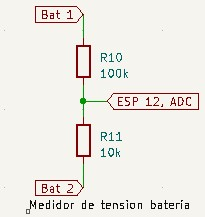
\includegraphics[width=0.5\linewidth]{hardware/Screenshot_16.jpg}
    \caption{Circuito de medición de baterías.}
    \label{fig:Vbat}
\end{figure}

El cruce por cero se mide con un circuito comparador (figura \ref{fig:cruce-cero}). Se toma la señal de alterna del transformador, y se compara con 0 constantemente. Cada vez que dicha señal cruce por cero, la salida de este circuito intercala flancos ascendentes y descendentes.\\

\begin{figure}[H]
    \centering
    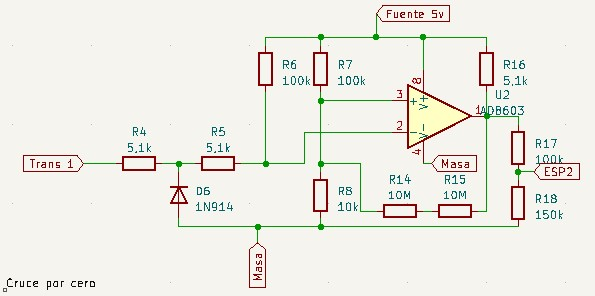
\includegraphics[width=0.9\linewidth]{hardware/Screenshot_15.jpg}
    \caption{Circuito cruce por cero.}
    \label{fig:cruce-cero}
\end{figure}

\begin{figure}[H]
    \centering
    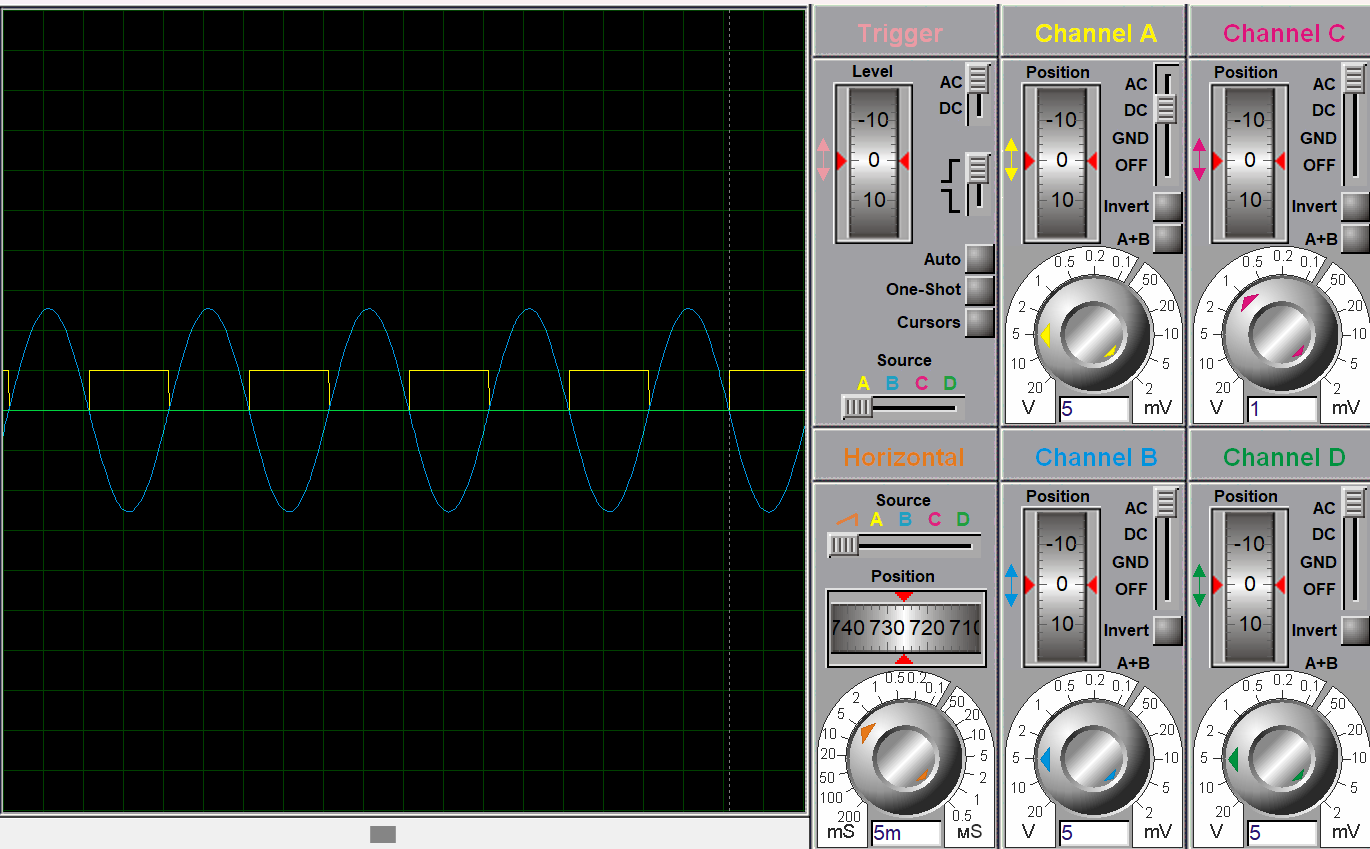
\includegraphics[width=1\linewidth]{hardware/Screenshot_26.png}
    \caption{Salida del circuito cruce por cero.}
    \label{fig:cruce,cero}
\end{figure}

\subsubsection{Alimentación}

La motherboard posee dos entradas de alimentación: batería ($\approx$12V dc) y transformador (9+9V ac).\\

Utilizando el mismo circuito que para alimentar el circuito de conmutación (figura \ref{fig:Fuente 12v}), el sistema puede seguir siendo utilizado frente a cortes en el suministro eléctrico. La motherboard posee un transformador exclusivo para que la lectura de tensión se vea lo menos afectada posible por consumos altos en la salida del mismo (estos provocan caídas en la tensión de salida).\\

Para alimentar el microcontrolador, junto al LCD de 20x04, y al ADC externo ADS1115, se requieren 5Vdc. Para esto, se utilizó un regulador de tensión LM7805, cuya entrada de almentación es la salida de la fuente de 12V, y su salida se conecta a los dispositivos mencionados. Además, la motherboard incluye una salida de 5V en una bornera, por si es necesario su uso en otro periférico.\\

\subsubsection{Resultado final}

\begin{figure}[H]
    \centering
    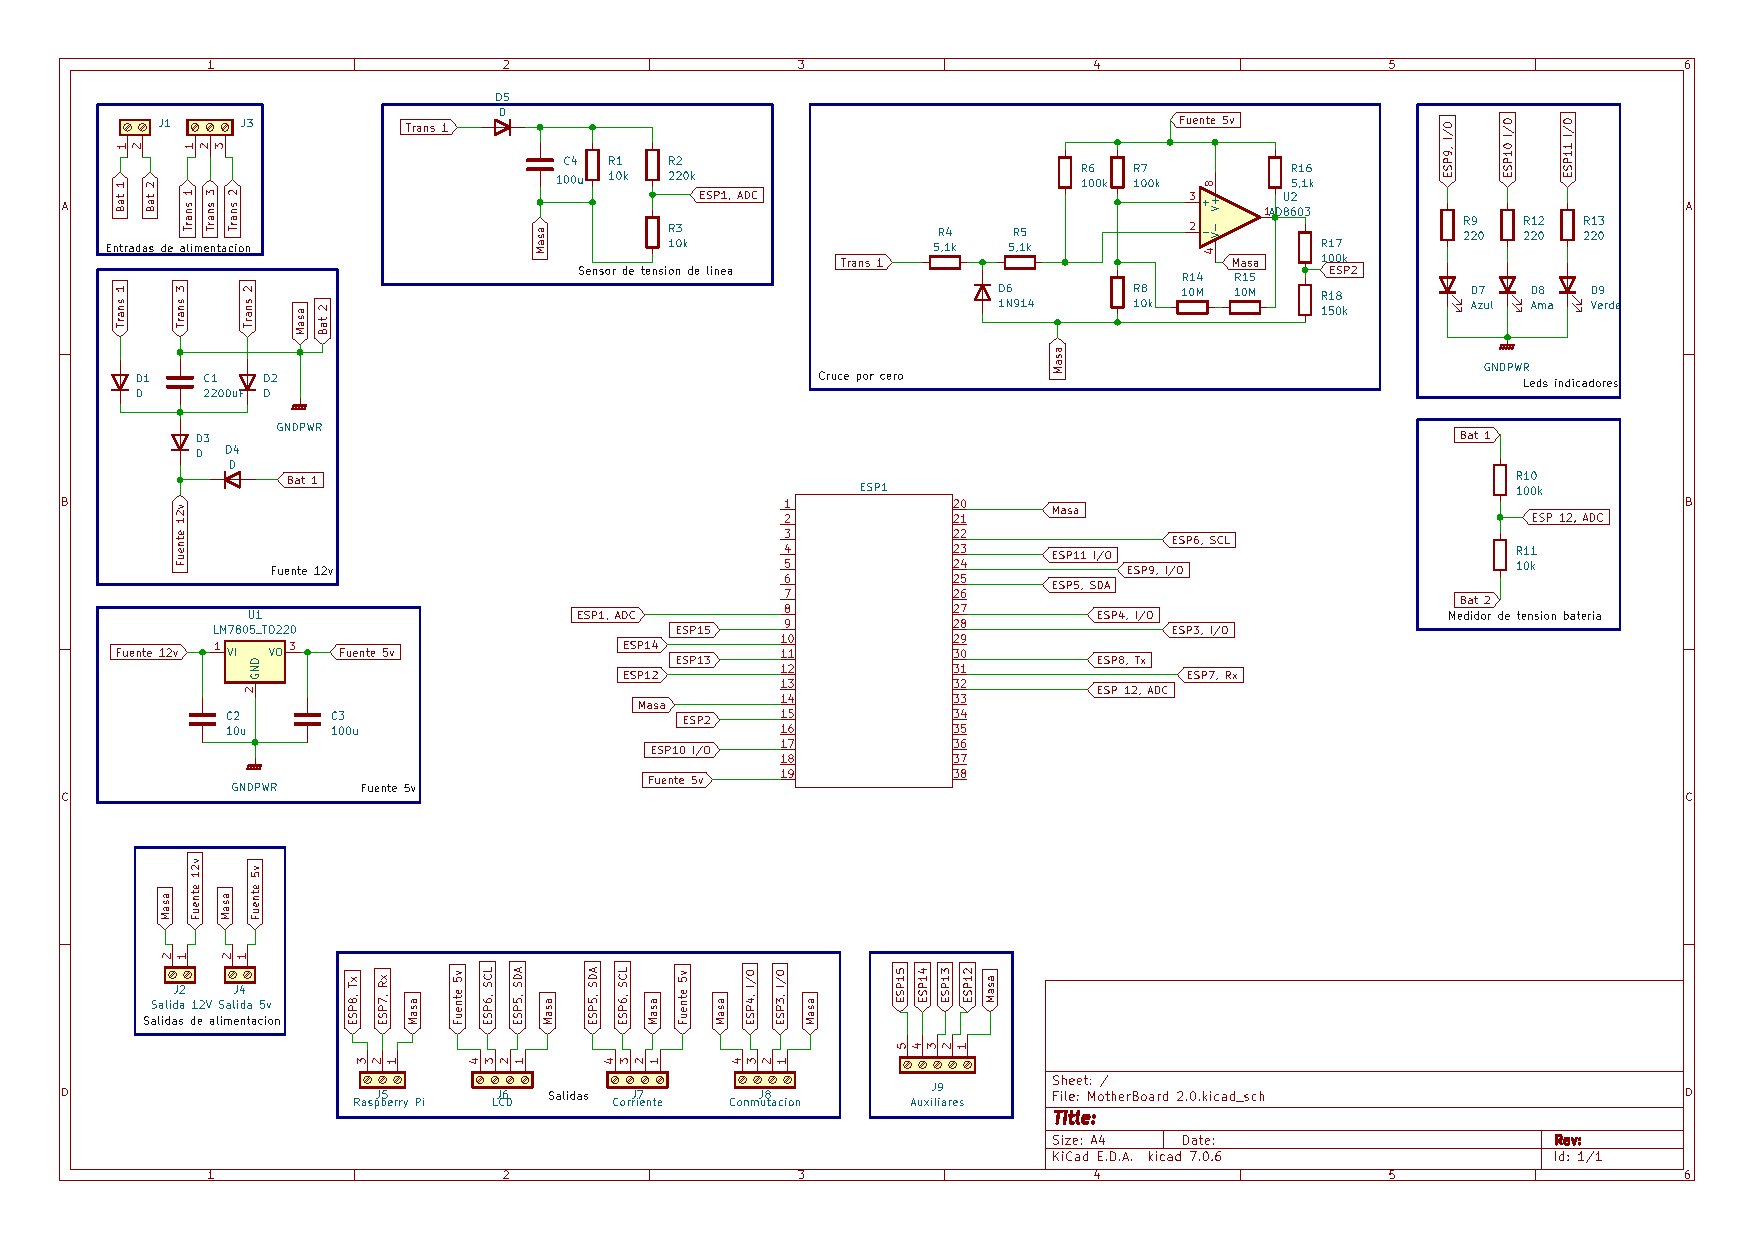
\includegraphics[width=1\linewidth]{hardware/MotherBoard 2.0.pdf}
    \caption{Diseño esquemático final de la motherboard.}
    \label{fig:mother-sch}
\end{figure}

\begin{figure}[H]
    \centering
    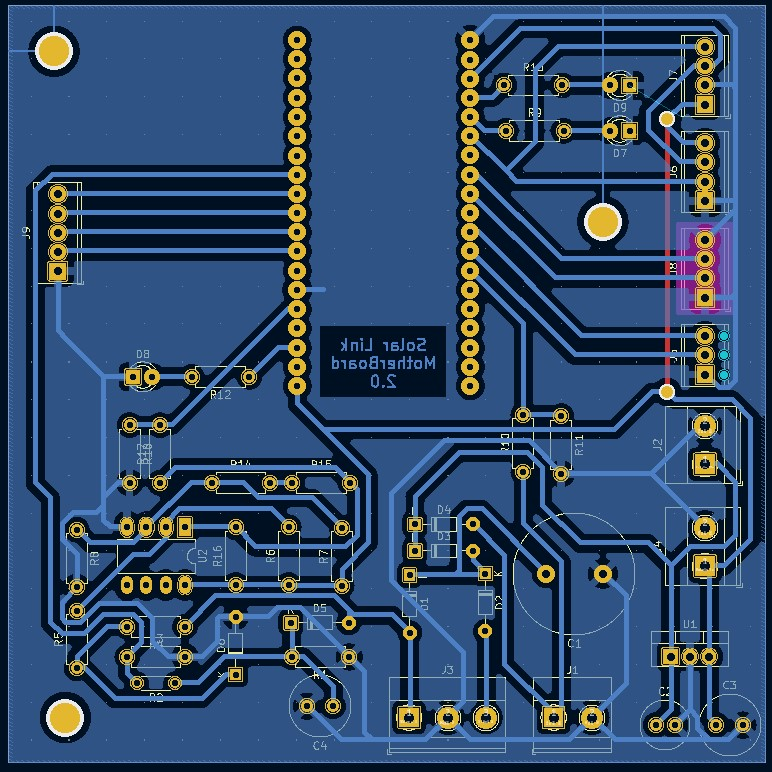
\includegraphics[width=0.7\linewidth]{hardware/Screenshot_17.jpg}
    \caption{Diseño del PCB final de la motherboard.}
    \label{fig:mother-pcb}
\end{figure}

\begin{figure}[H]

\begin{subfigure}{0.5\textwidth}
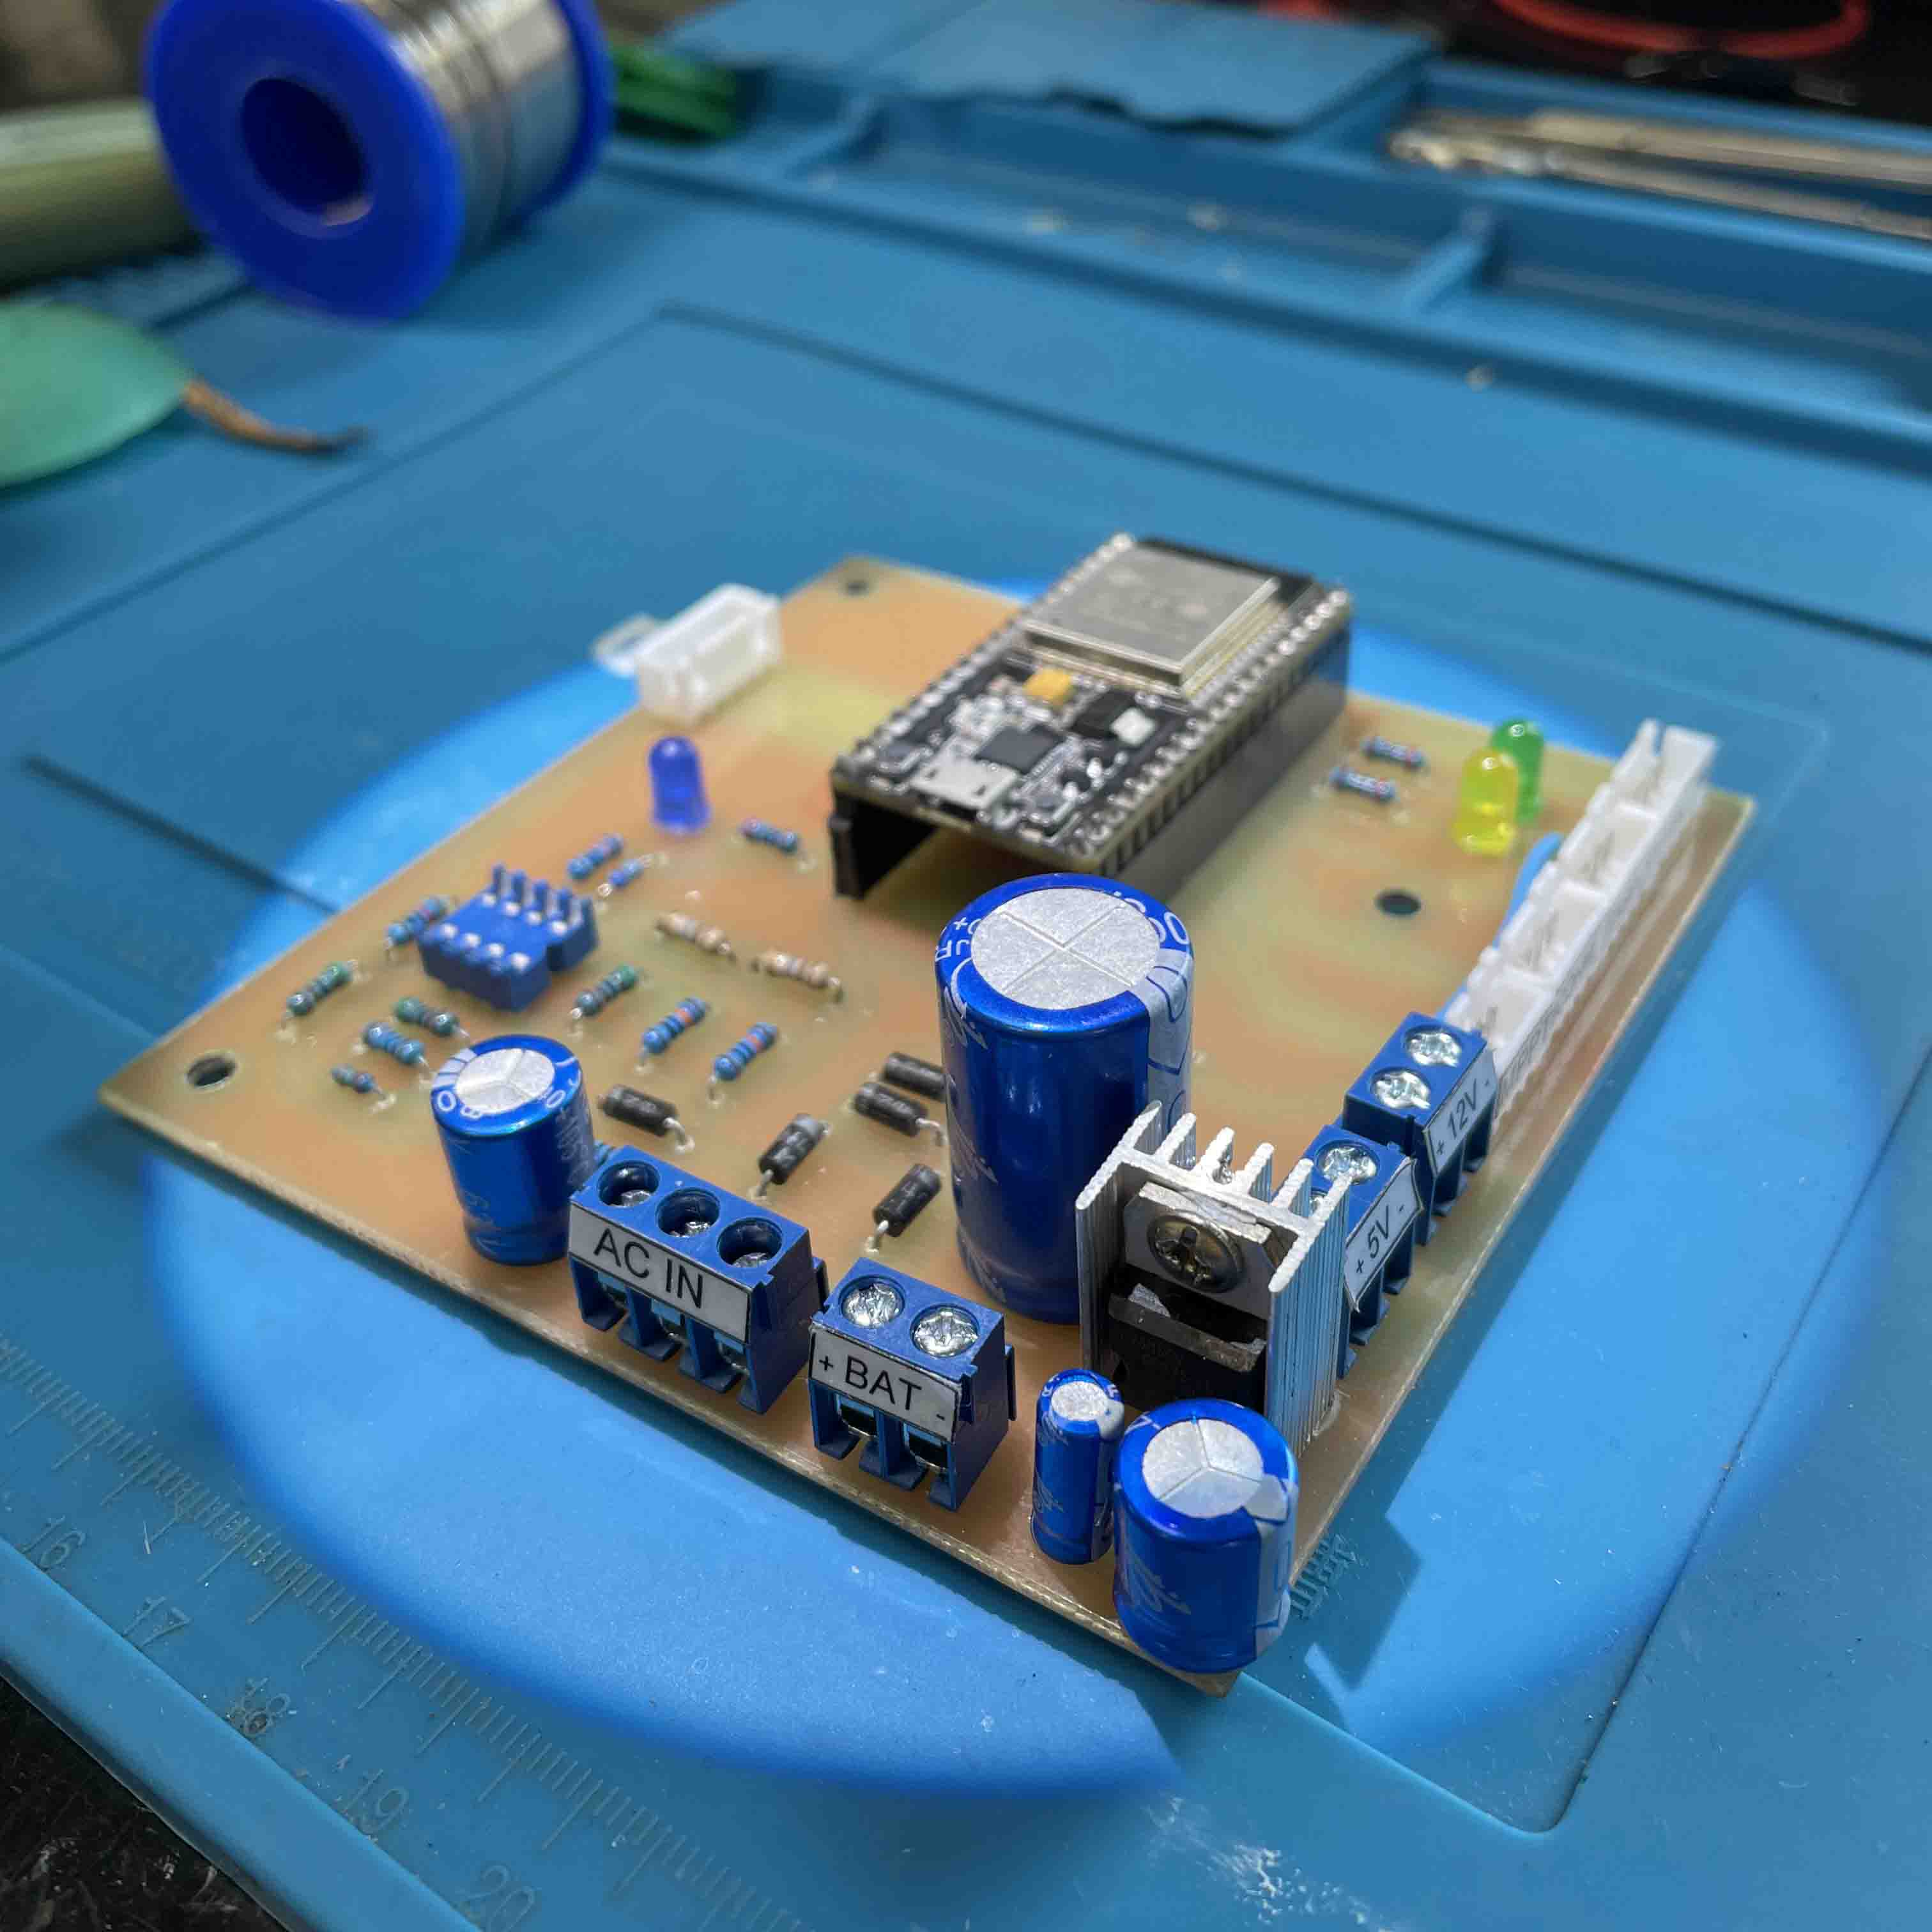
\includegraphics[width=0.9\linewidth]{hardware/IMG_8945.jpg} 
\caption{Plaqueta final motherboard.}
\label{fig:corr-fin}
\end{subfigure}
\begin{subfigure}{0.5\textwidth}
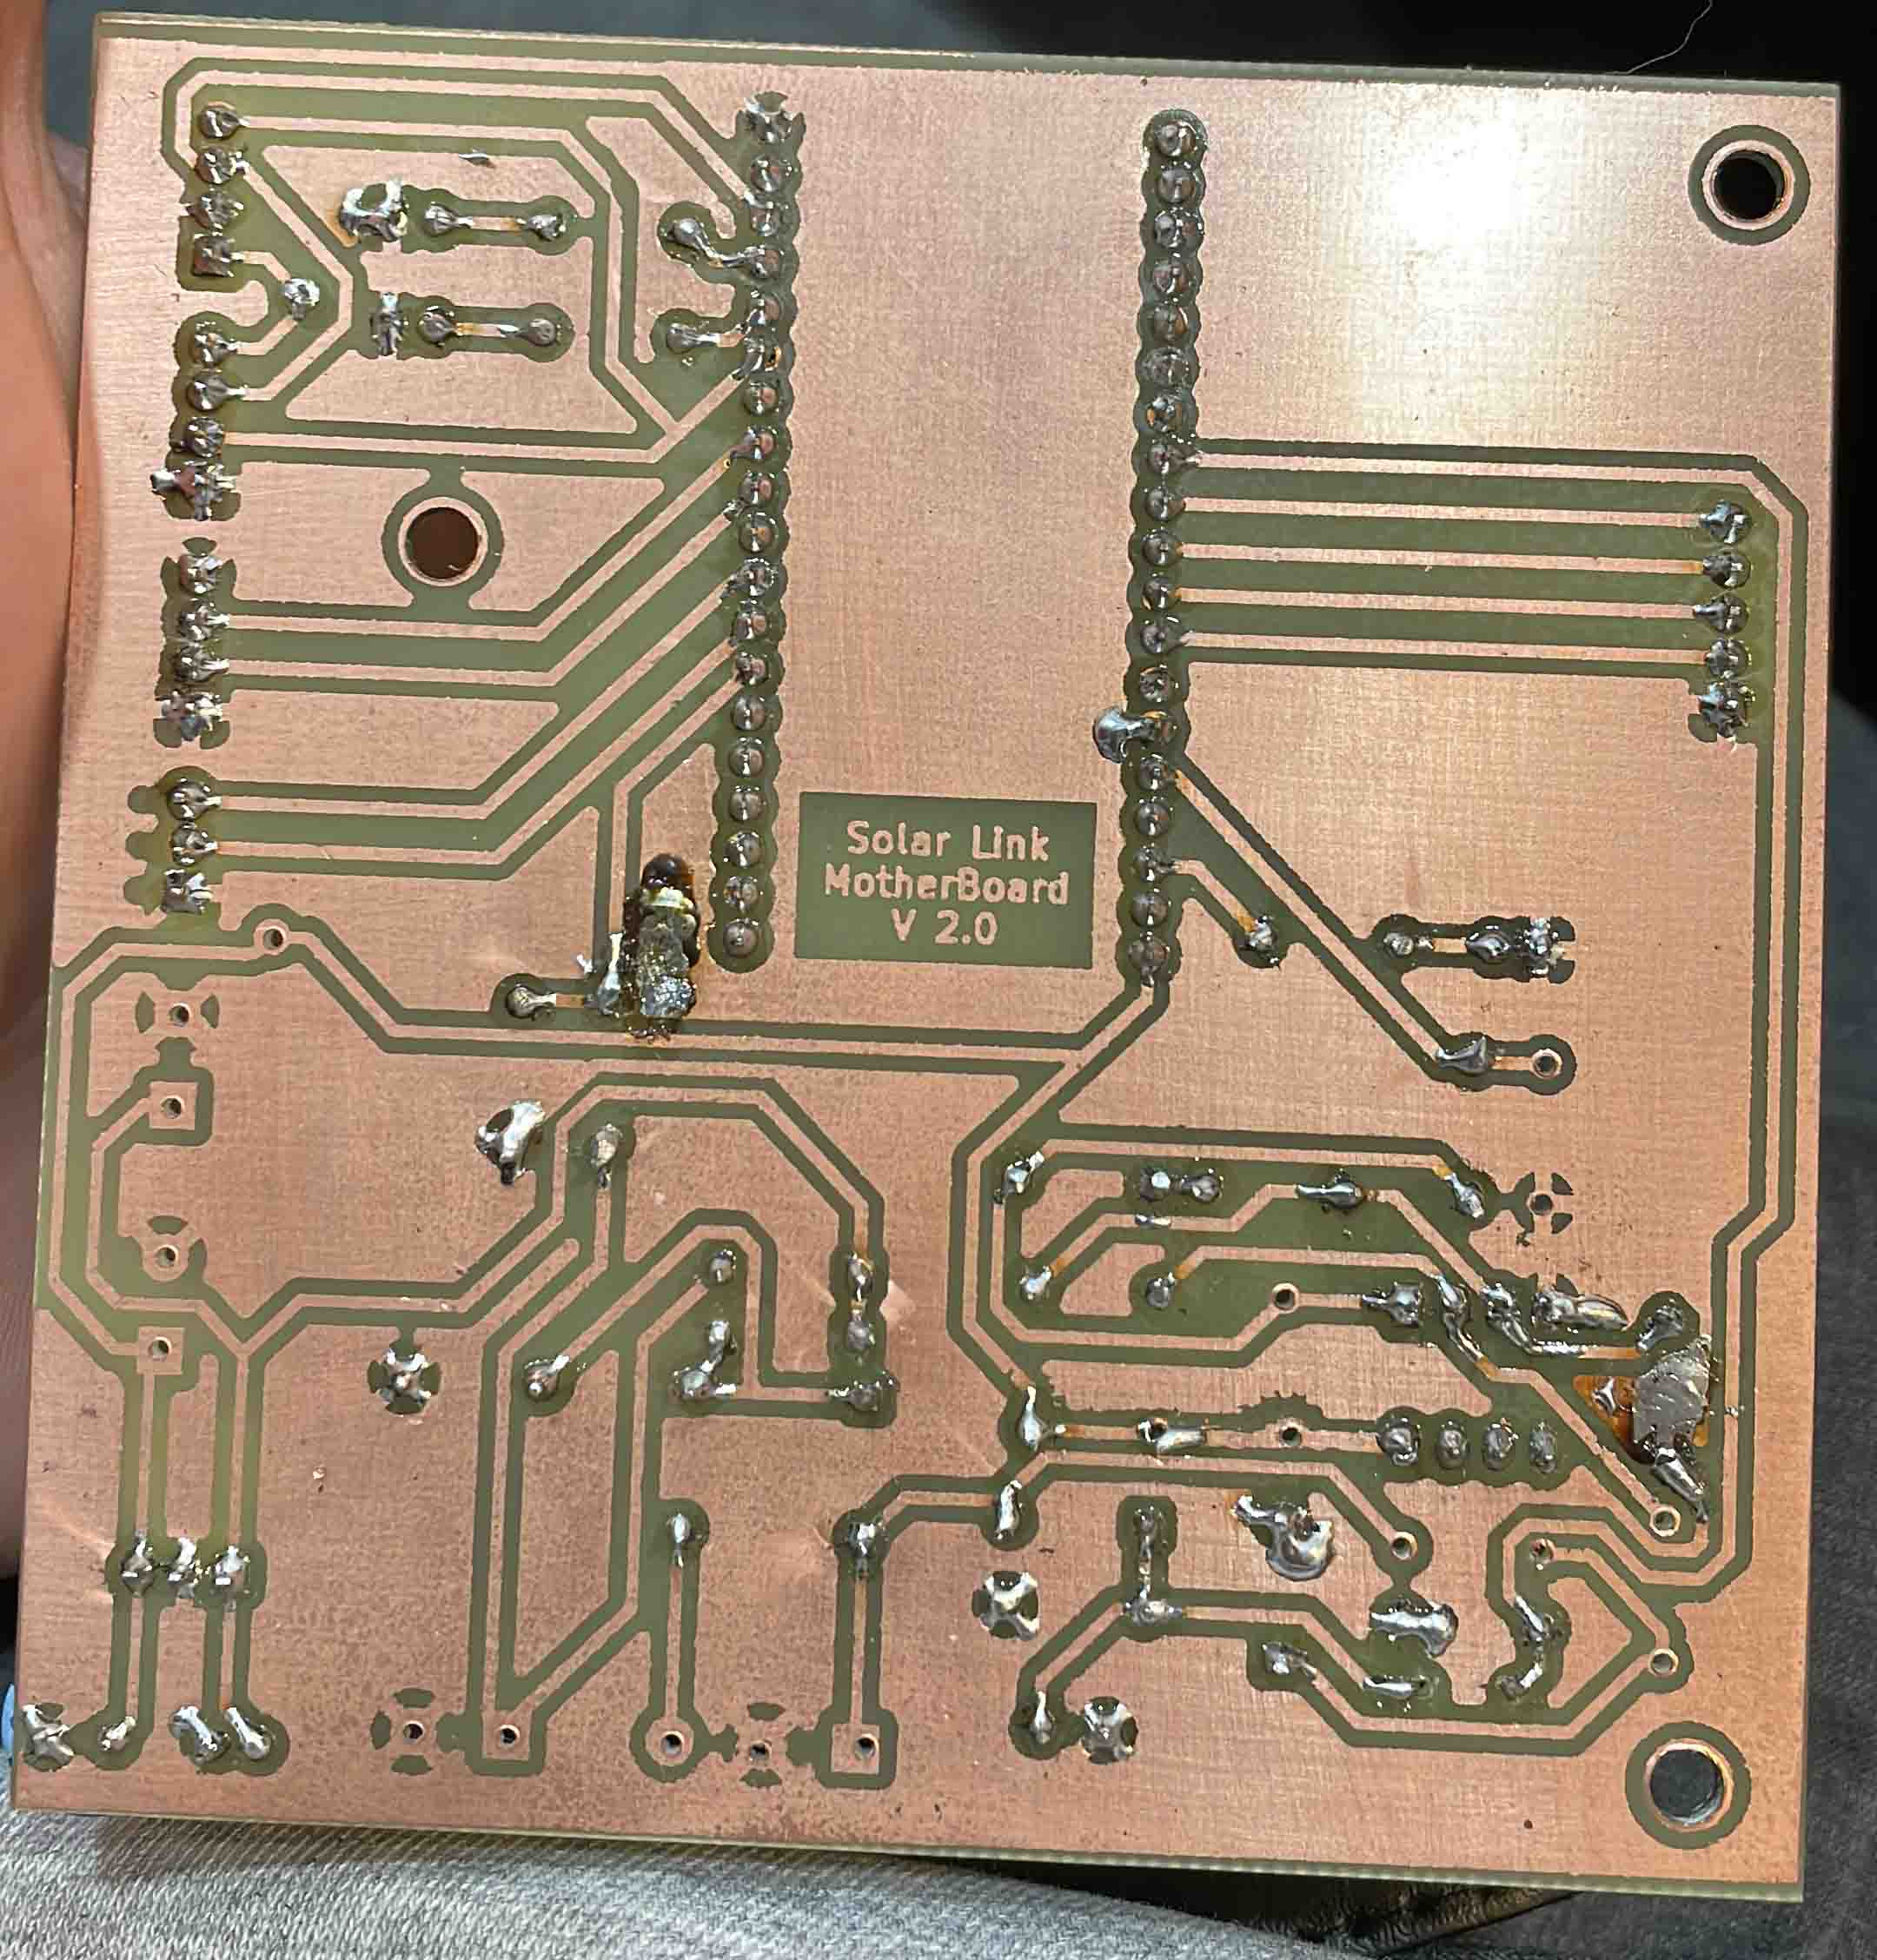
\includegraphics[width=0.9\linewidth]{hardware/F44CD098-7B36-40C0-95DB-D5040B6878EF.JPG}
\caption{Plaqueta motherboard lado inferior.}
\label{fig:corr-pcb}
\end{subfigure}

\caption{Resultados finales de la motherboard.}
\label{fig:corriente-fin}
\end{figure}

\subsection{Medidor de corriente}

\subsubsection{Explicación del circuito}

Para medir la corriente, utilizamos los sensores HW-666, cuya principal ventaja es que son no invasivos. Esto quiere decir que no tenemos que intervenir directamente en la línea eléctrica para realizar las mediciones.\\

\begin{wrapfigure}{l}{0.3\textwidth}
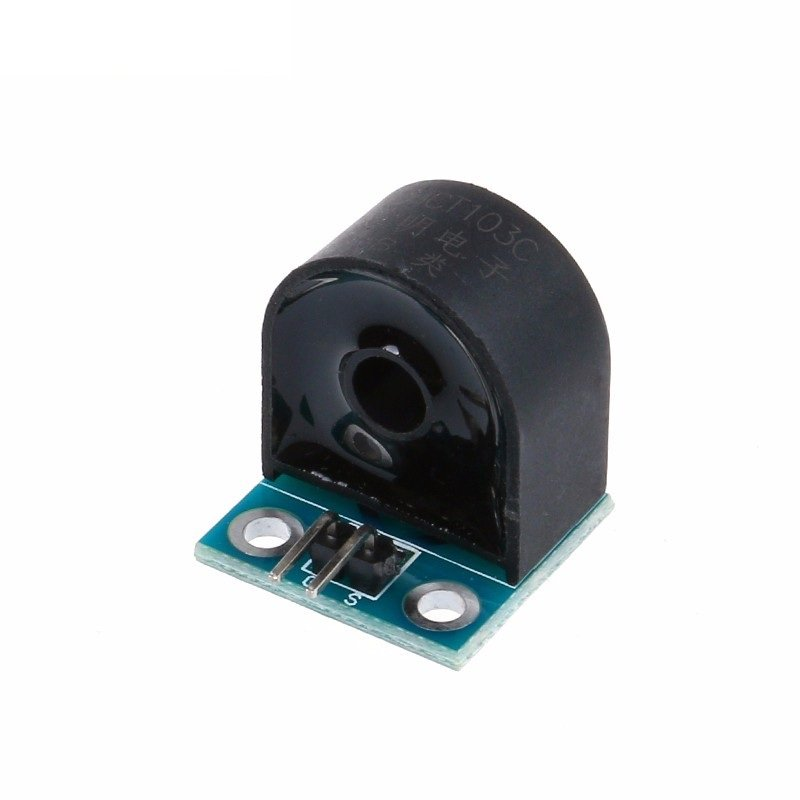
\includegraphics[width=0.9\linewidth]{hardware/hw666.jpg} 
\caption{Sensor de corriente HW-666}
\label{fig:hw666}
\end{wrapfigure}

Estos sensores son unos transformadores de corriente con una relación de vueltas de 1000:1. Cuando se le introduce un cable por su orificio, la corriente que circule en este será inducida en el sensor. Como tiene en paralelo una resistencia de 100$\Omega$, la corriente inducida en el transformador circulará por la resistencia, resultando en un voltaje proporcional.\\

% \begin{wrapfigure}{b}{0.3\textwidth}
% 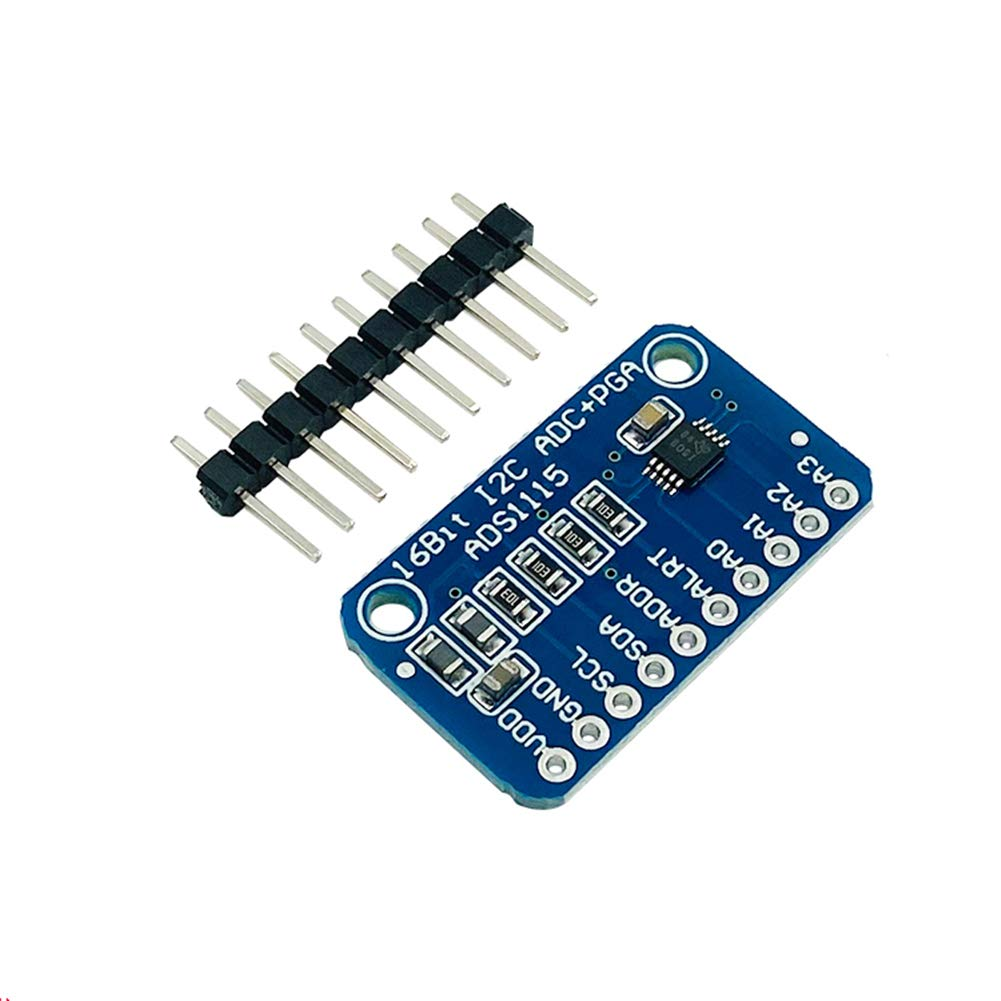
\includegraphics[width=0.9\linewidth]{hardware/ads1115.jpg} 
% \caption{ADC externo ADS1115}
% \label{fig:ads1115}
% \end{wrapfigure}

El voltaje que devuelve el sensor es de una señal alterna, que varía entre semiciclos positivos y negativos. Por lo tanto, para medir esta señal se requiere de un ADC diferencial, que permite la medición tanto de voltajes positivos como negativos.\\

Para esto utilizamos el ADC externo ADS1115, de 16 bits de resolución, que posee 4 entradas de ADC, pudiendo utilizarlas de a pares en modo diferencial, es decir, 2 entradas de ADC diferencial.\\

\begin{figure}[H]
    \centering
    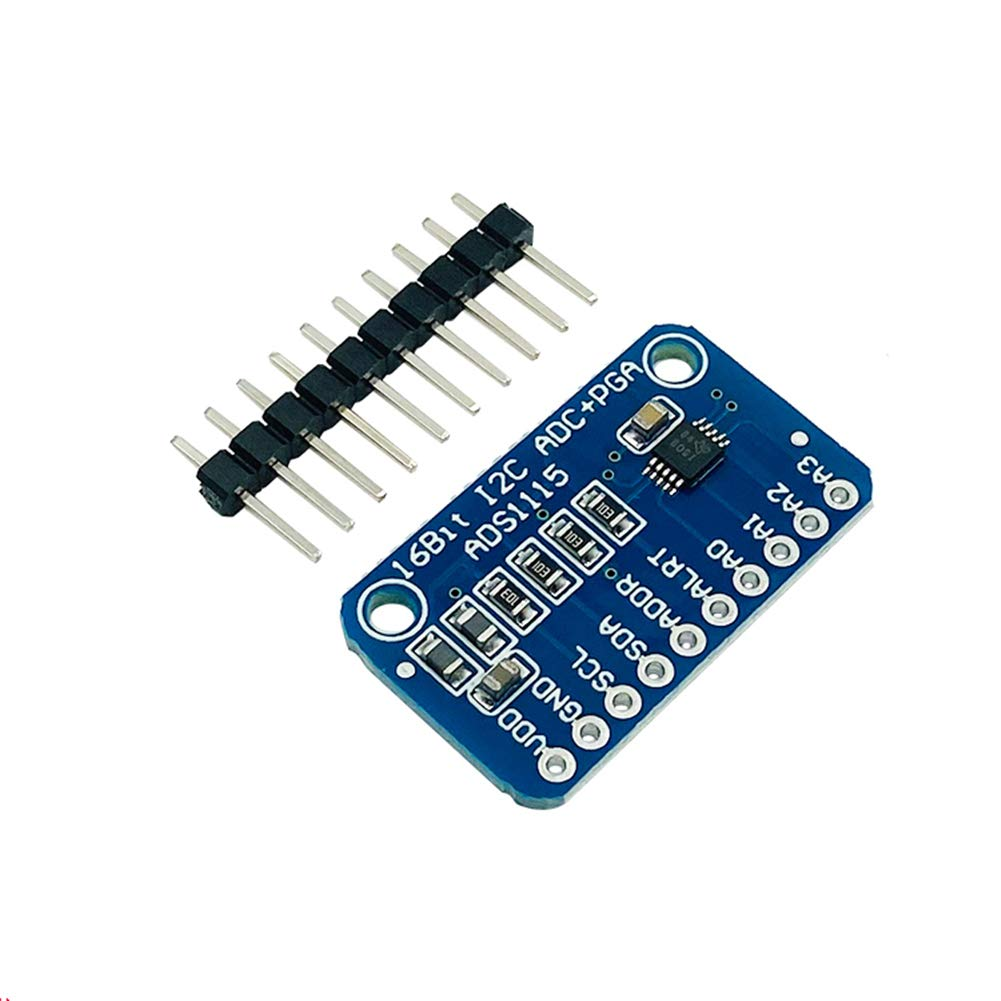
\includegraphics[width=0.5\linewidth]{hardware/ads1115.jpg}
    \caption{ADC externo ADS1115}
    \label{fig:ads1115}
\end{figure}

Este ADC procesa la señal y se la transmite al microcontrolador a través del protocolo de comunicación I2C.\\

\subsubsection{Resultado final}

\begin{figure}[H]
    \centering
    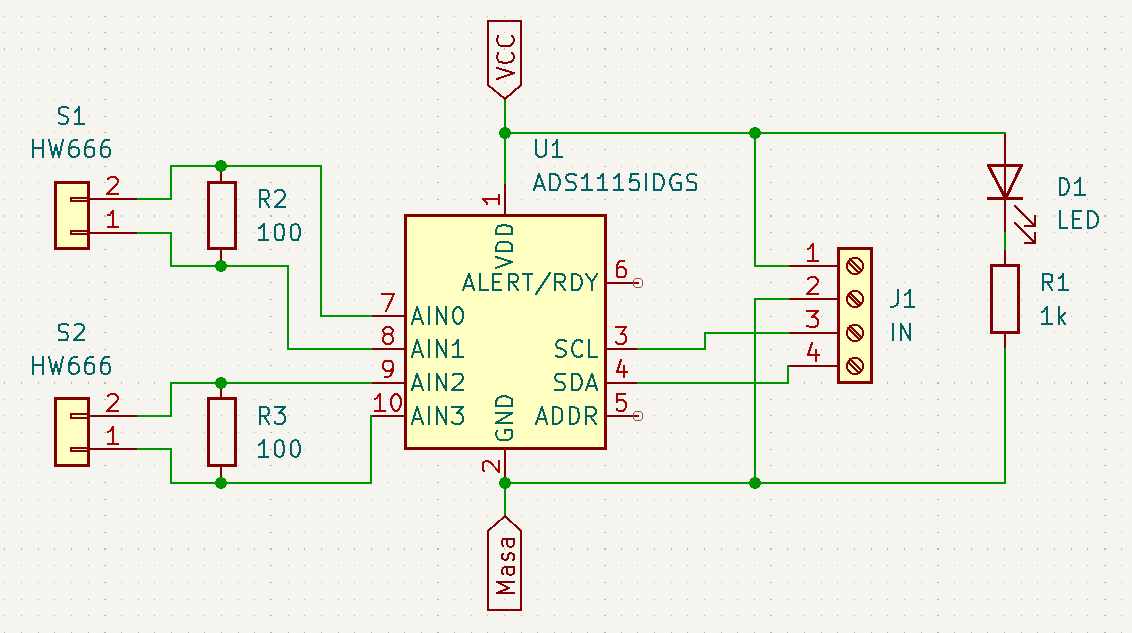
\includegraphics[width=0.9\linewidth]{hardware/Screenshot_11.png}
    \caption{Diseño de esquemático.}
    \label{fig:sch-corr}
\end{figure}

\begin{figure}[H]
    \centering
    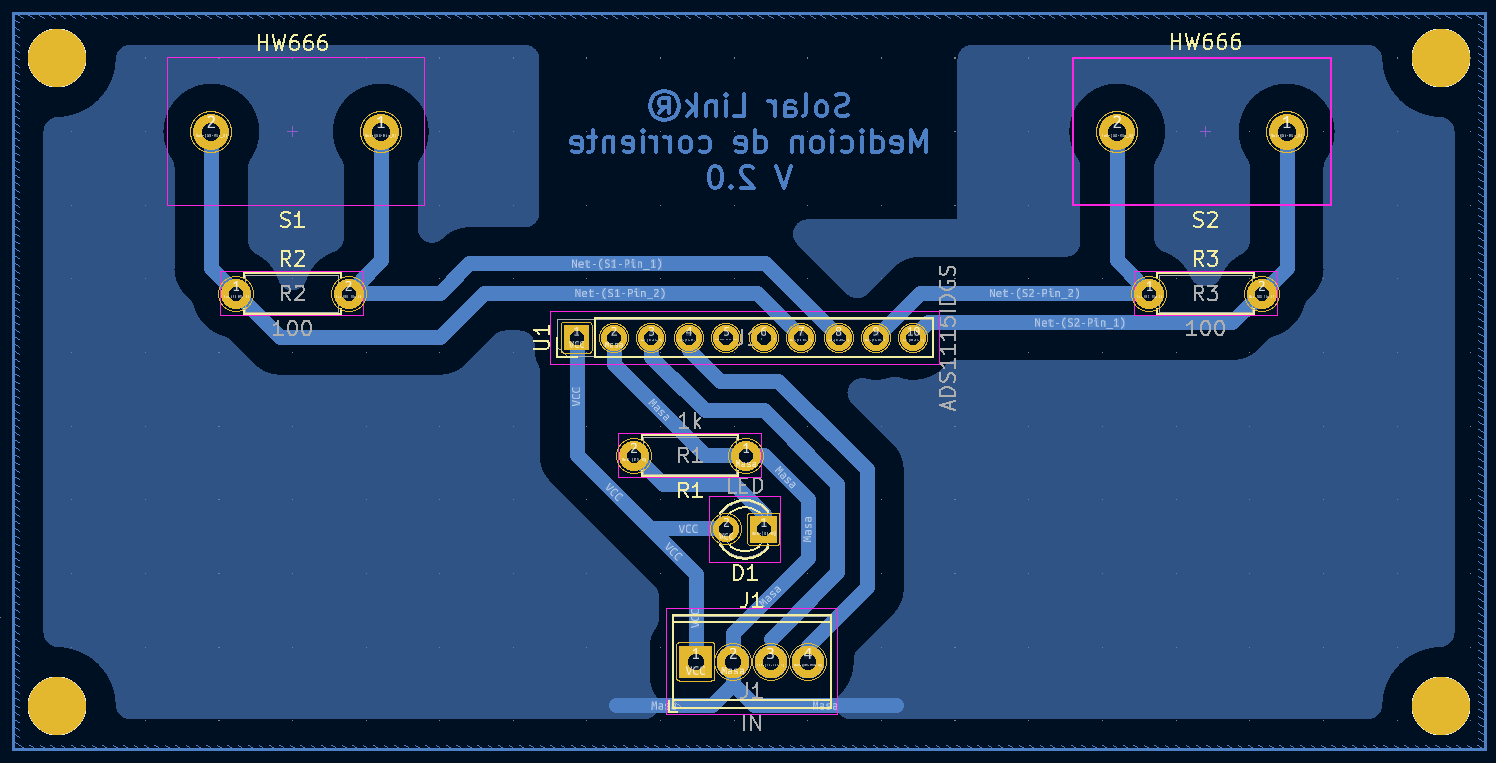
\includegraphics[width=0.9\linewidth]{hardware/Screenshot_12.png}
    \caption{Diseño de PCB.}
    \label{fig:pcb-corr}
\end{figure}

\begin{figure}[H]

\begin{subfigure}{0.5\textwidth}
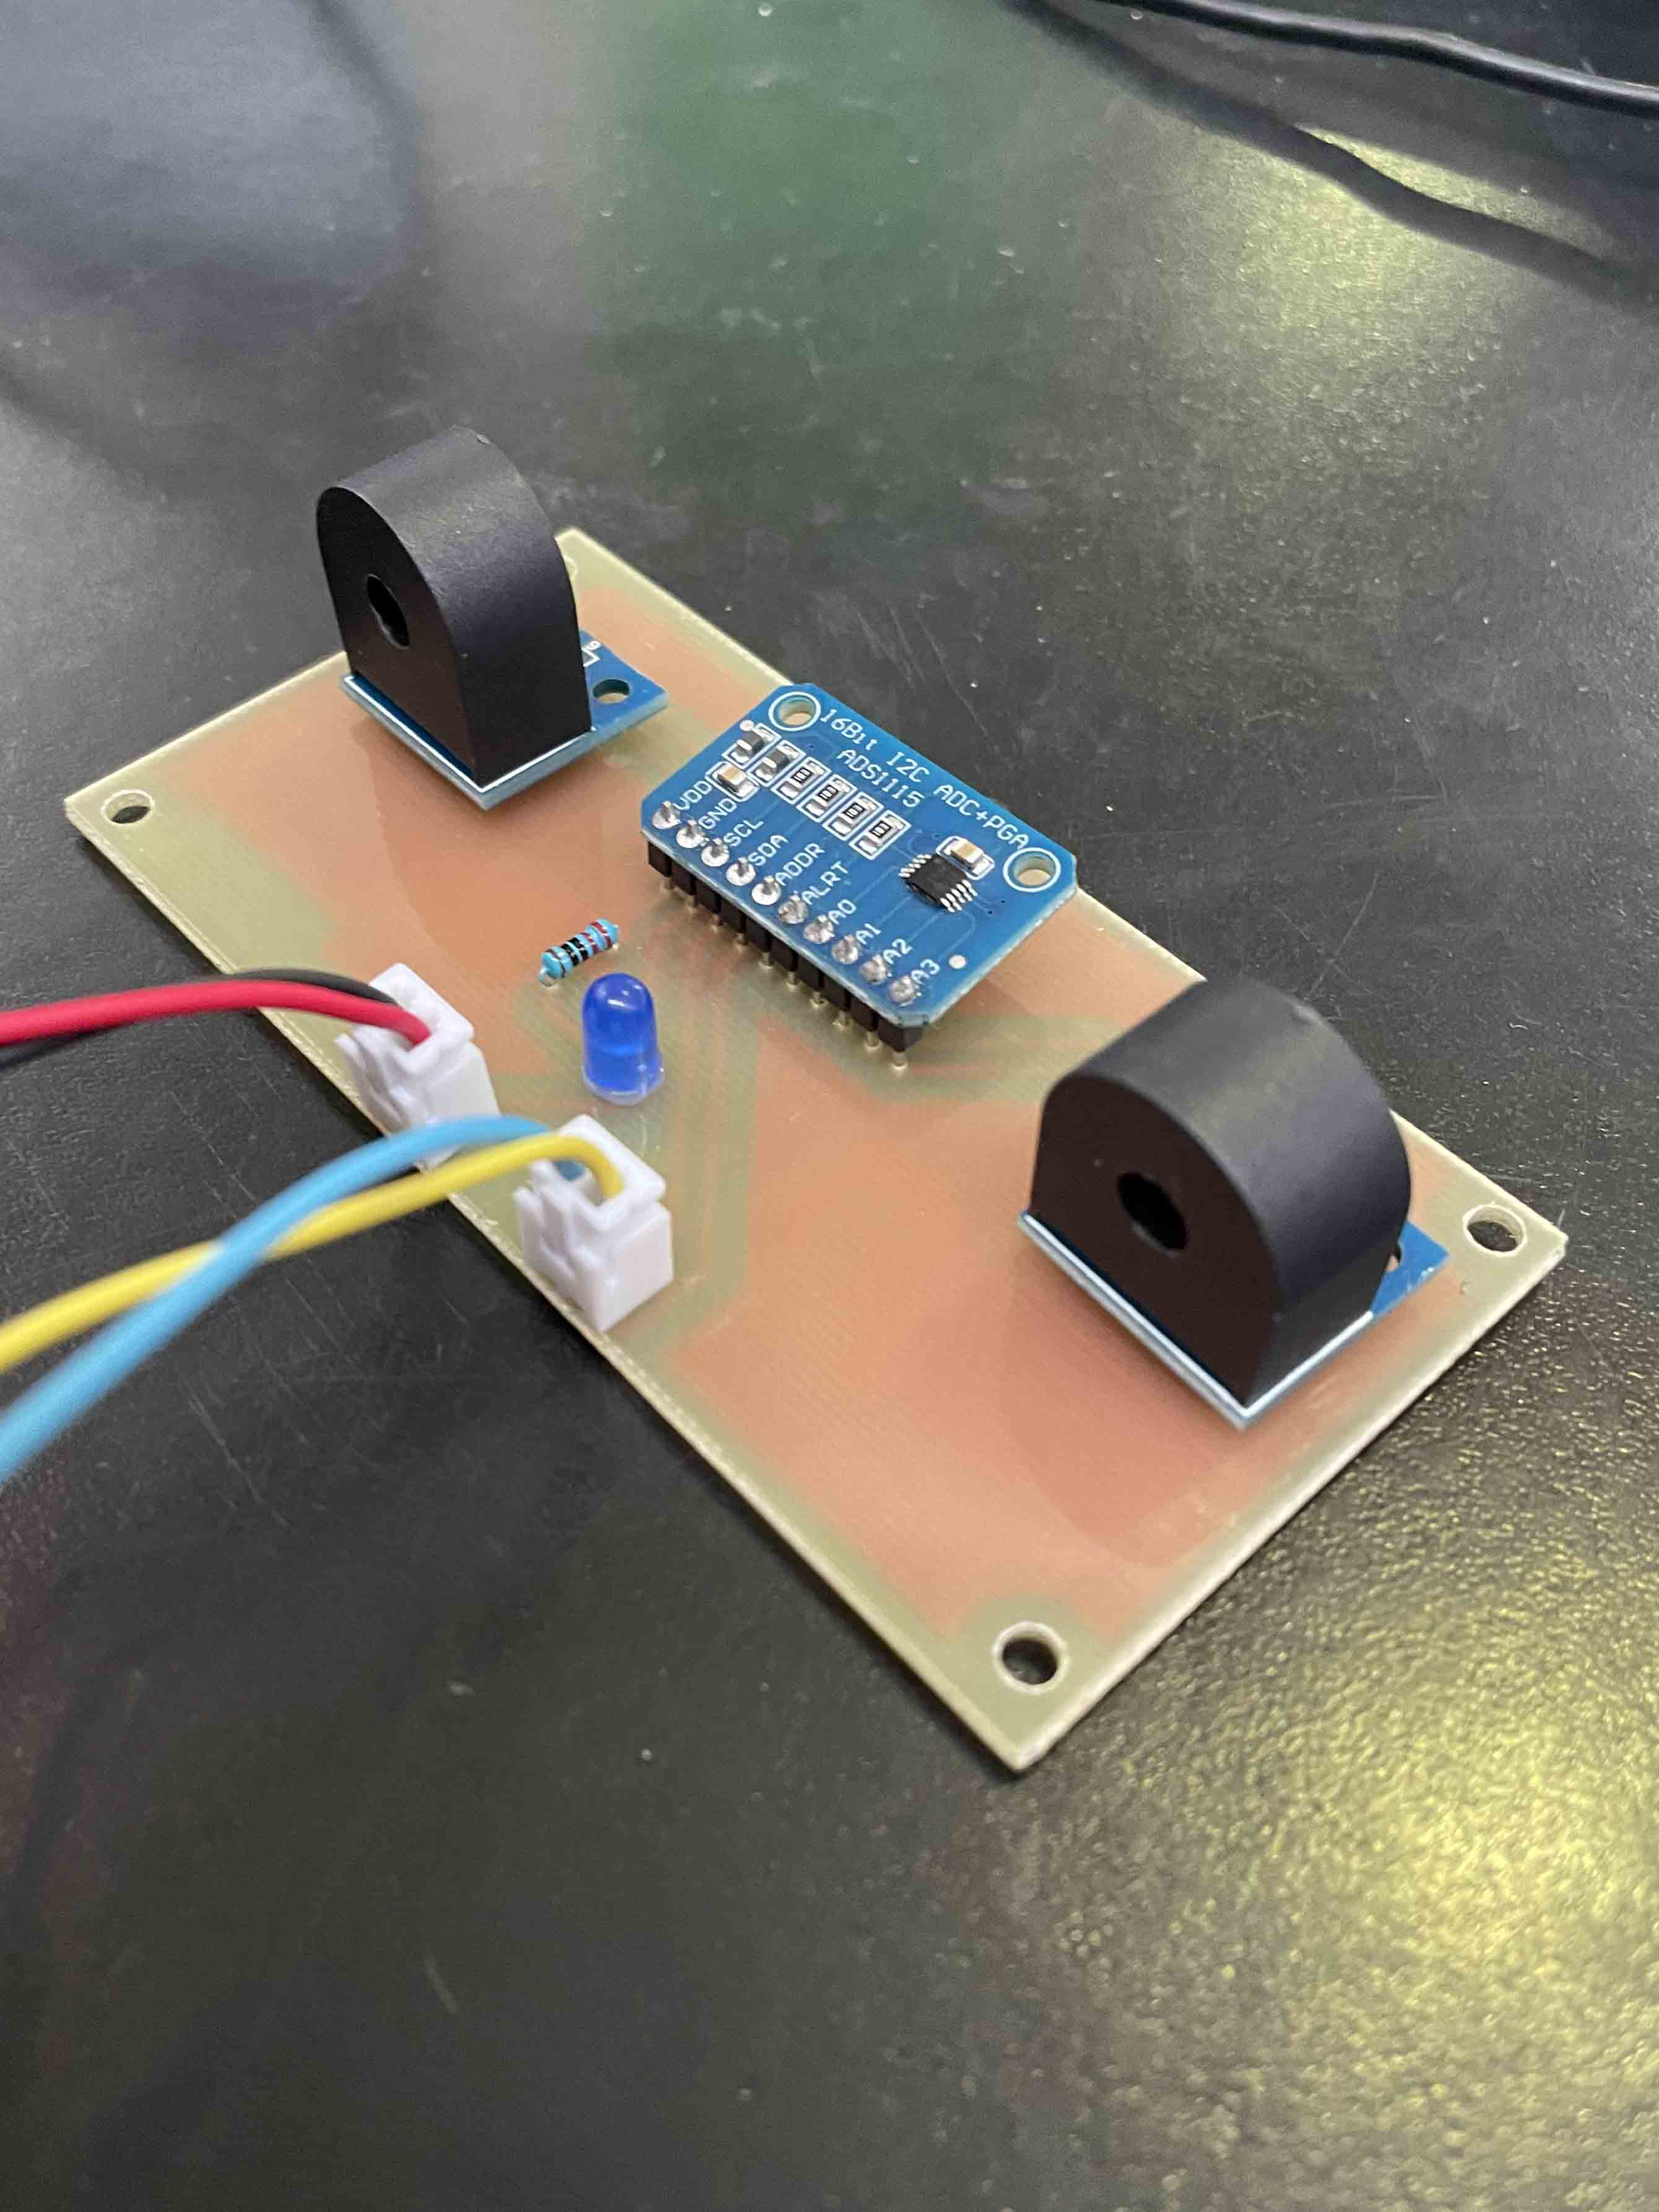
\includegraphics[width=0.9\linewidth]{hardware/IMG_8066.jpg} 
\caption{Plaqueta final medidor de \\corriente.}
\label{fig:corr-fin}
\end{subfigure}
\begin{subfigure}{0.5\textwidth}
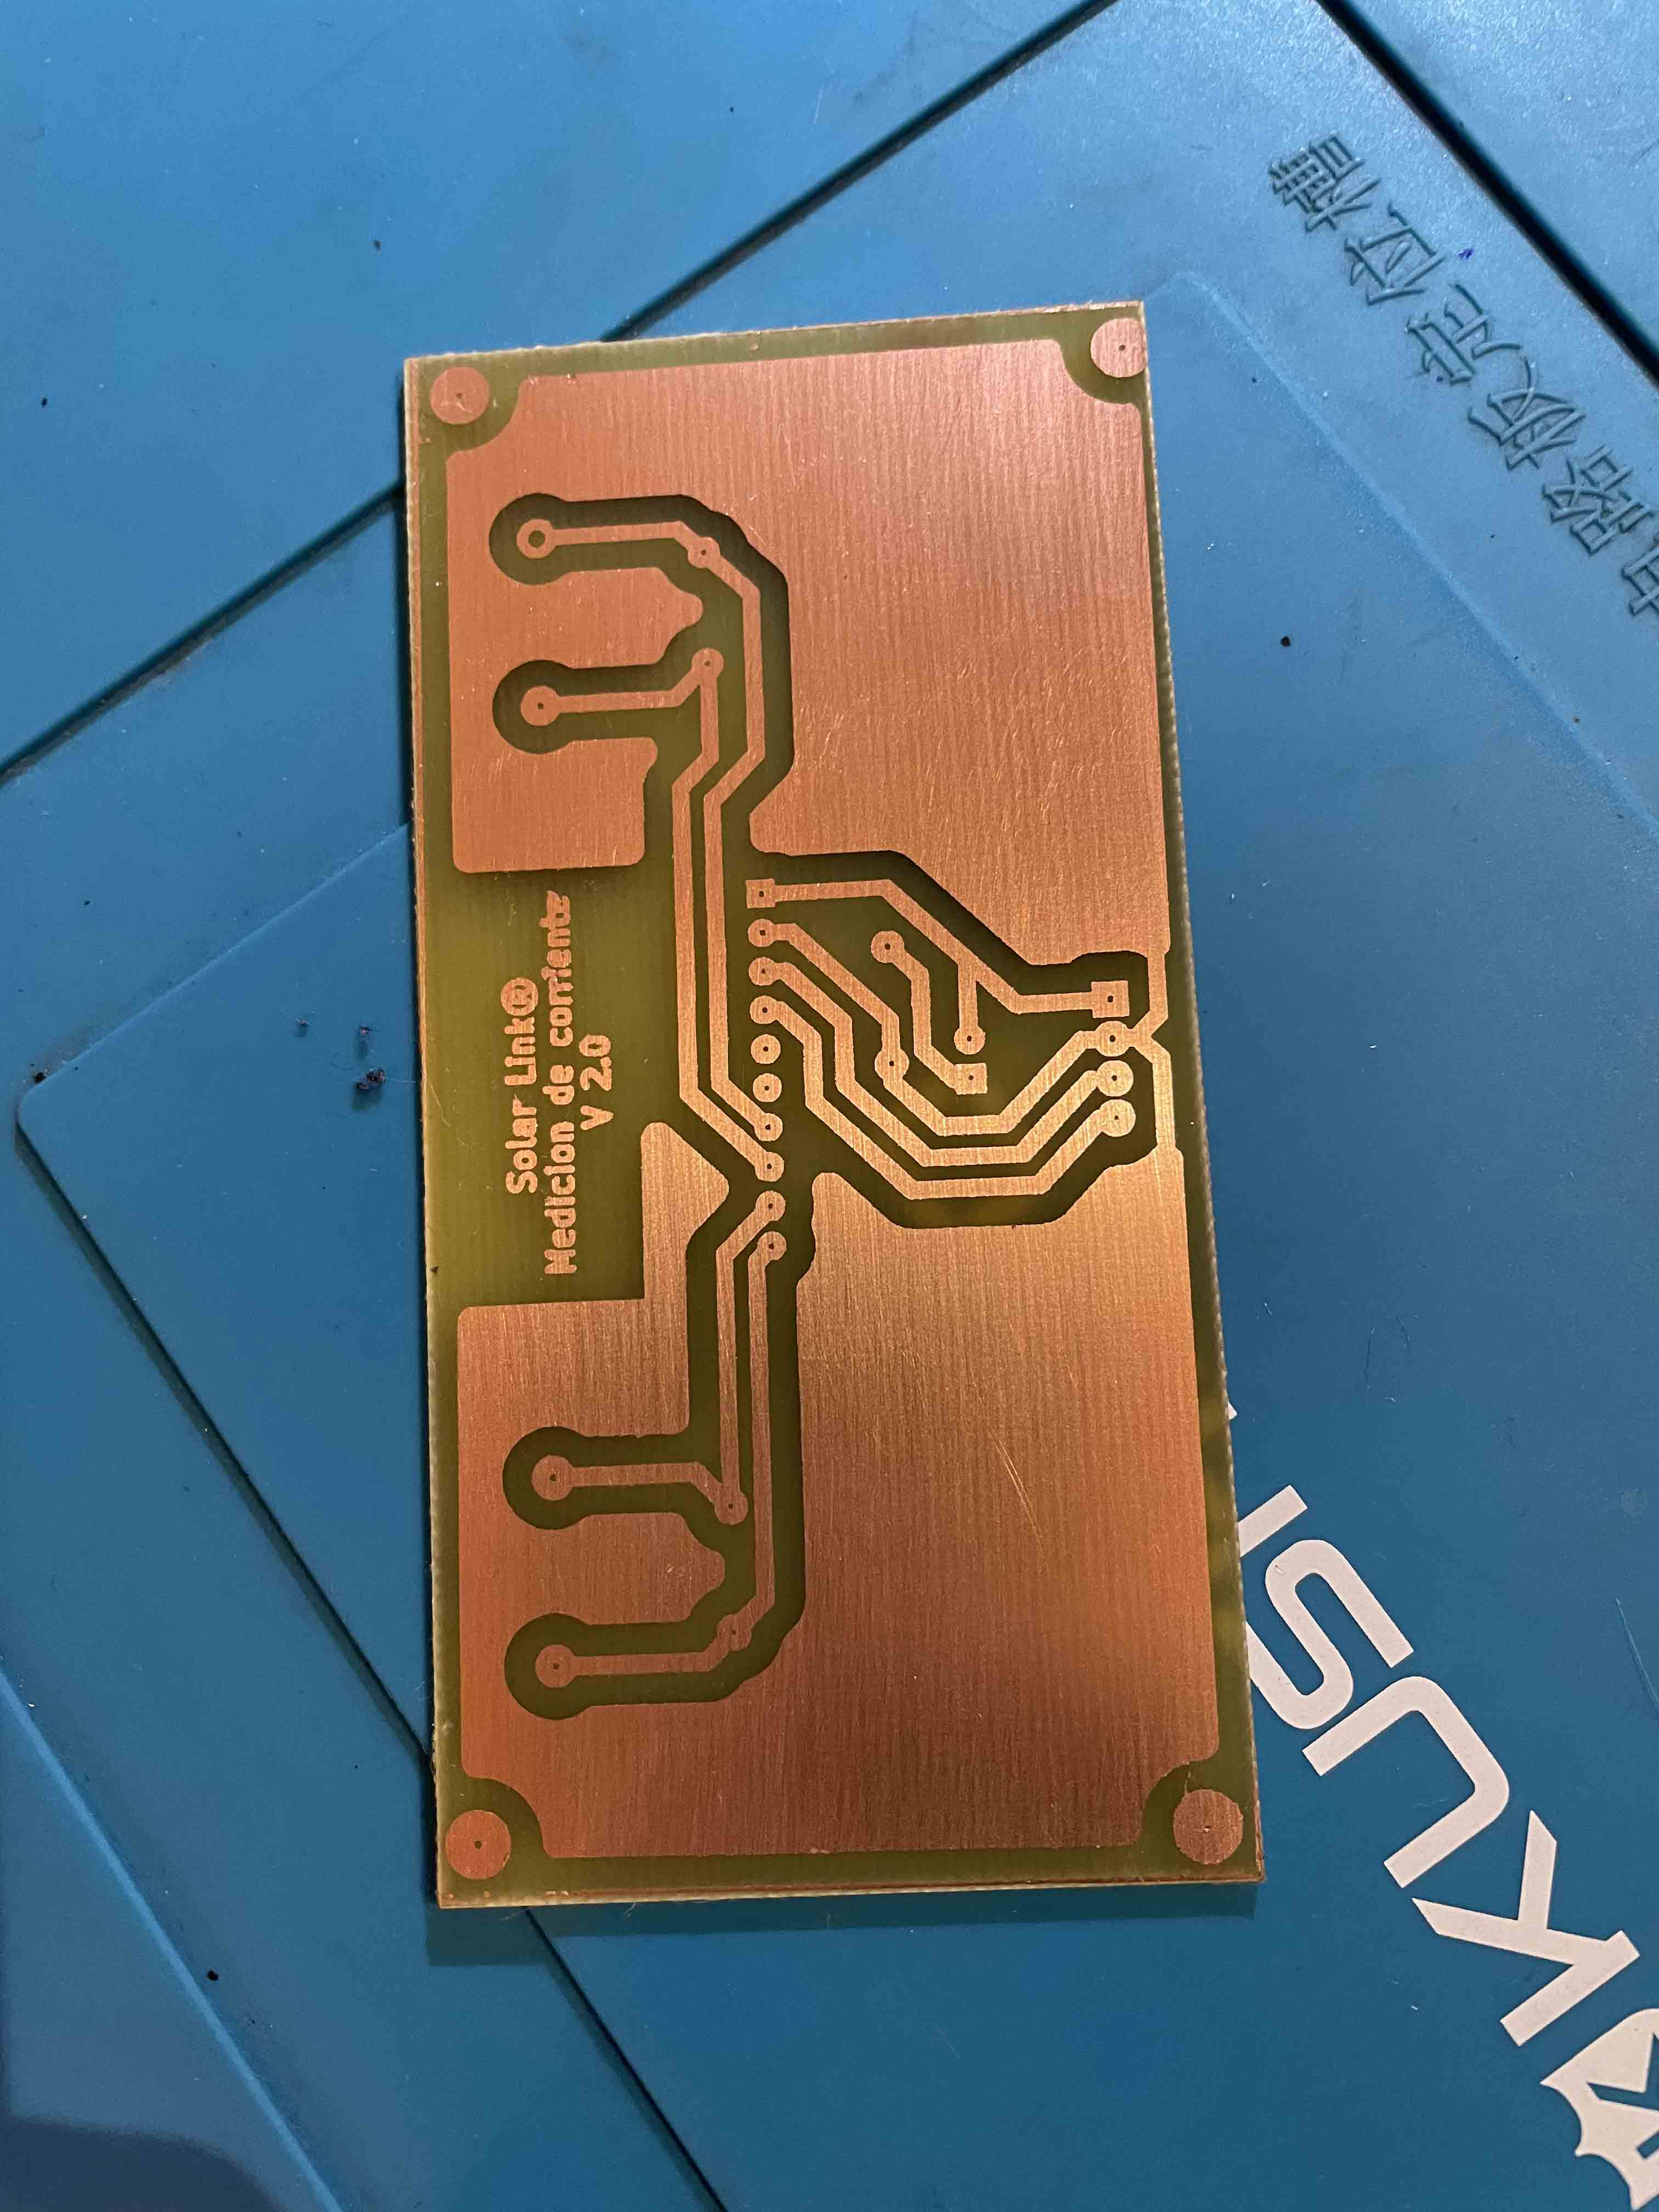
\includegraphics[width=0.9\linewidth]{hardware/IMG_8587.jpg}
\caption{Plaqueta final medidor de corriente \\lado inferior.}
\label{fig:corr-pcb}
\end{subfigure}

\caption{Resultados finales del medidor de corriente.}
\label{fig:corriente-fin}
\end{figure}

Con una correcta calibración, resulta ser un módulo de medición muy preciso tanto en pequeñas como grandes escalas. Como lo estipula el fabricante, la máxima corriente que puede medir sin empezar a dar valores erróneos ronda en los 10A.

\clearpage

\subsection{Módulo de conmutación}

\subsubsection{Explicación del circuito}

Para conmutar entre líneas utilizamos los relés de potencia inversores HJQ-15F-S-Z, que con un simple pulso nos permite cambiar entre sus terminales normal cerrado y normal abierto.\\

\begin{figure}[H]
    \centering
    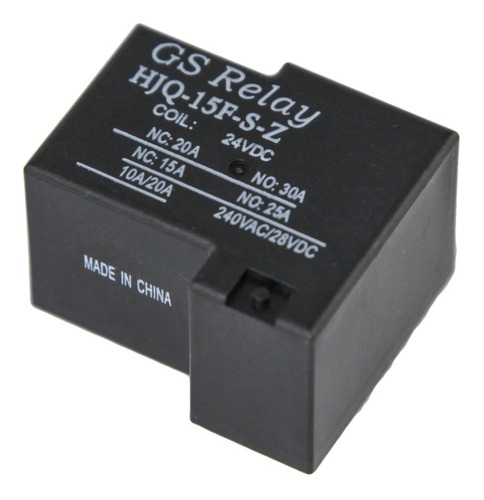
\includegraphics[width=0.4\linewidth]{hardware/Rele.jpg}
    \caption{Relé HJQ-15F-S-Z}
    \label{fig:rele}
\end{figure}

Para conmutar estos relés, fue necesario utilizar el circuito de la figura \ref{fig:opto-mosfet-rele}. Este circuito cuenta con un MOSFET IRFZ44N encargado de conmutar la alimentación de la bobina del relé, y un optoacoplador para alimentar el gate del MOSFET con la señal entrante del ESP32. \\

\begin{figure}[H]
    \centering
    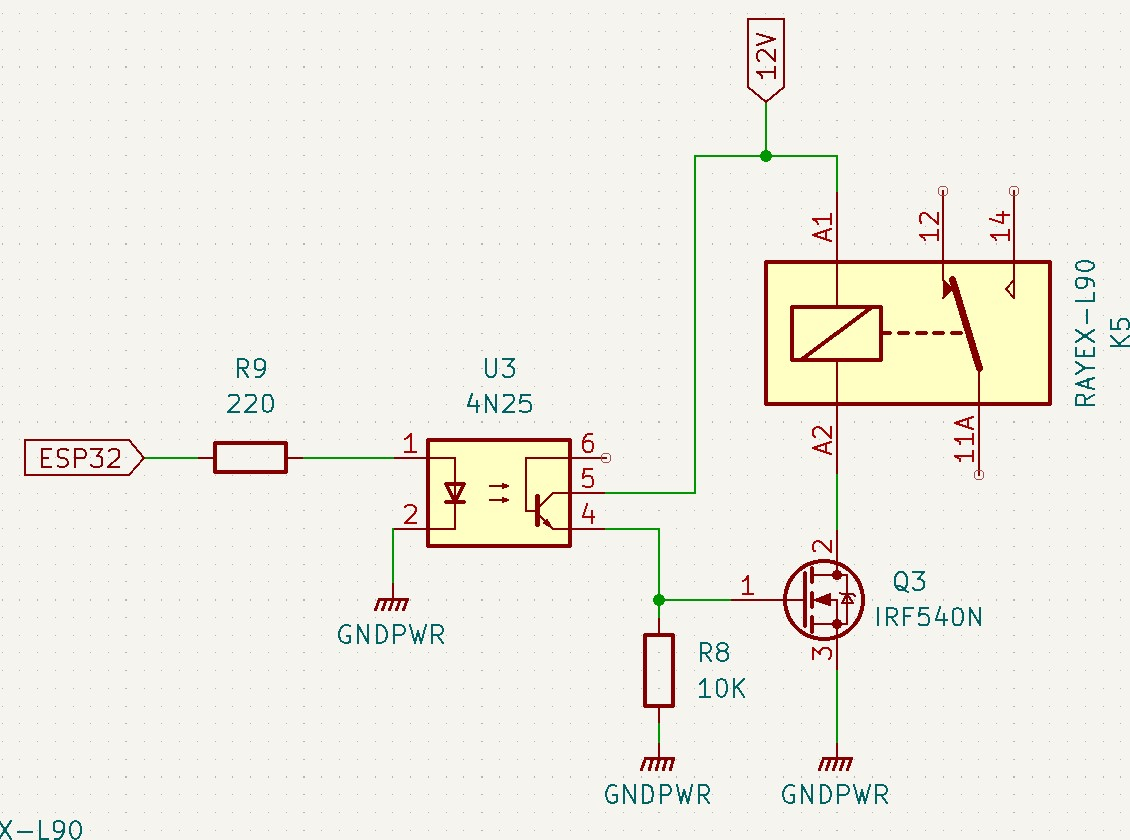
\includegraphics[width=0.9\linewidth]{hardware/Screenshot_19.jpg}
    \caption{Circuito de conmutación.}
    \label{fig:opto-mosfet-rele}
\end{figure}

Utilizamos el optoacoplador para aislar el microcontrolador del circuito de potencia. En caso de una falla eléctrica, el ESP32 no se vería afectado y seguiría funcionando sin problema.\\

\subsubsection{Resultado final}

\begin{figure}[H]
    \centering
    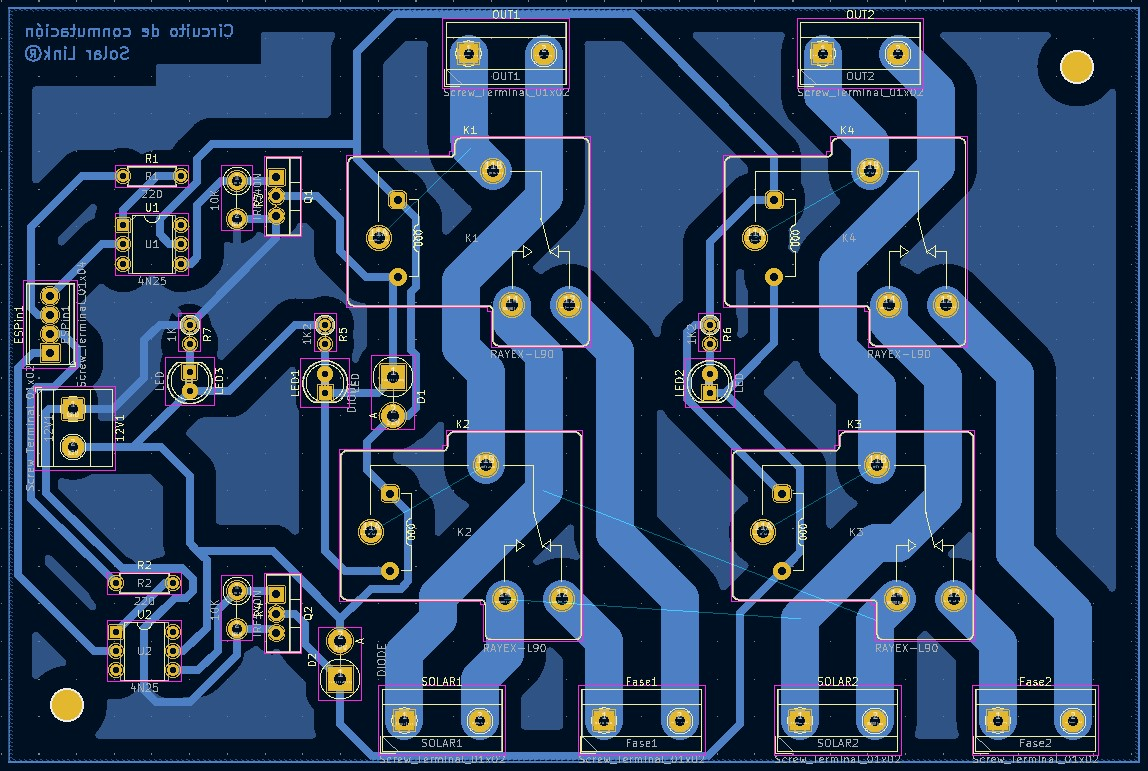
\includegraphics[width=1\linewidth]{hardware/Screenshot_18.jpg}
    \caption{Diseño final PCB de conmutación.}
    \label{fig:conmutacion-pcb}
\end{figure}

\begin{figure}[H]

\begin{subfigure}{0.5\textwidth}
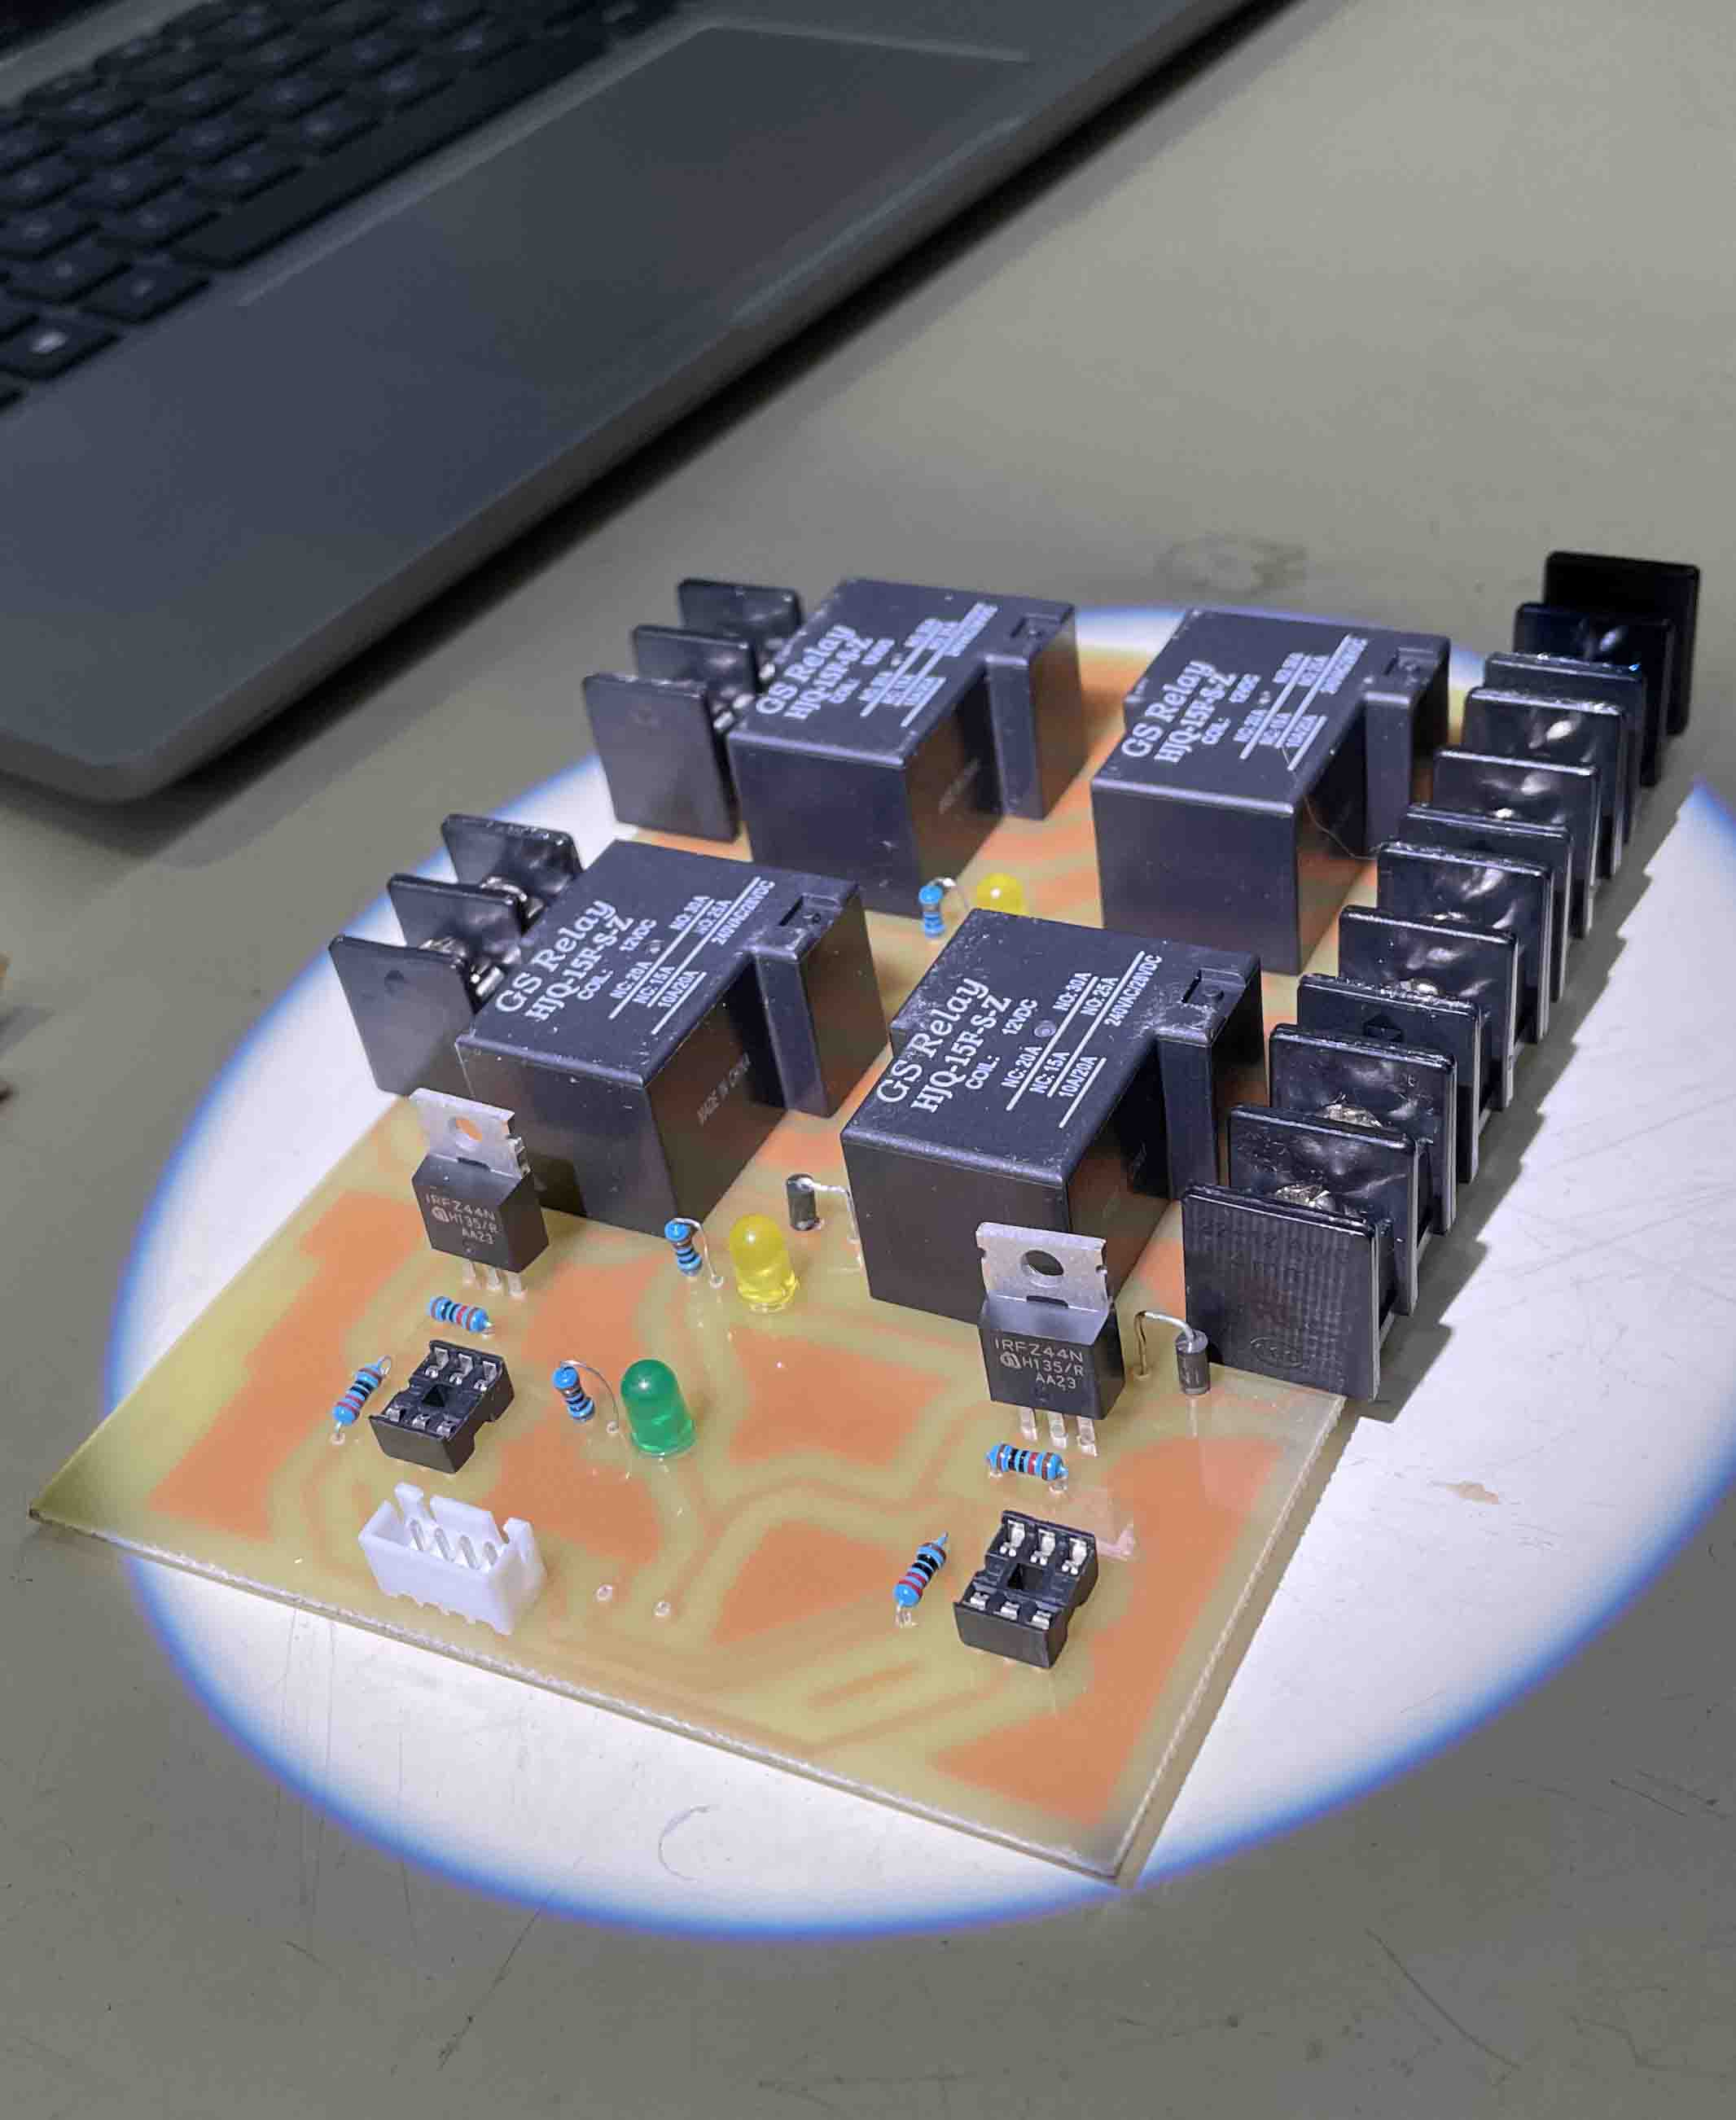
\includegraphics[width=0.9\linewidth]{hardware/IMG_8220.jpg} 
\caption{PCB final de conmutación.}
\label{fig:conm-fin}
\end{subfigure}
\begin{subfigure}{0.5\textwidth}
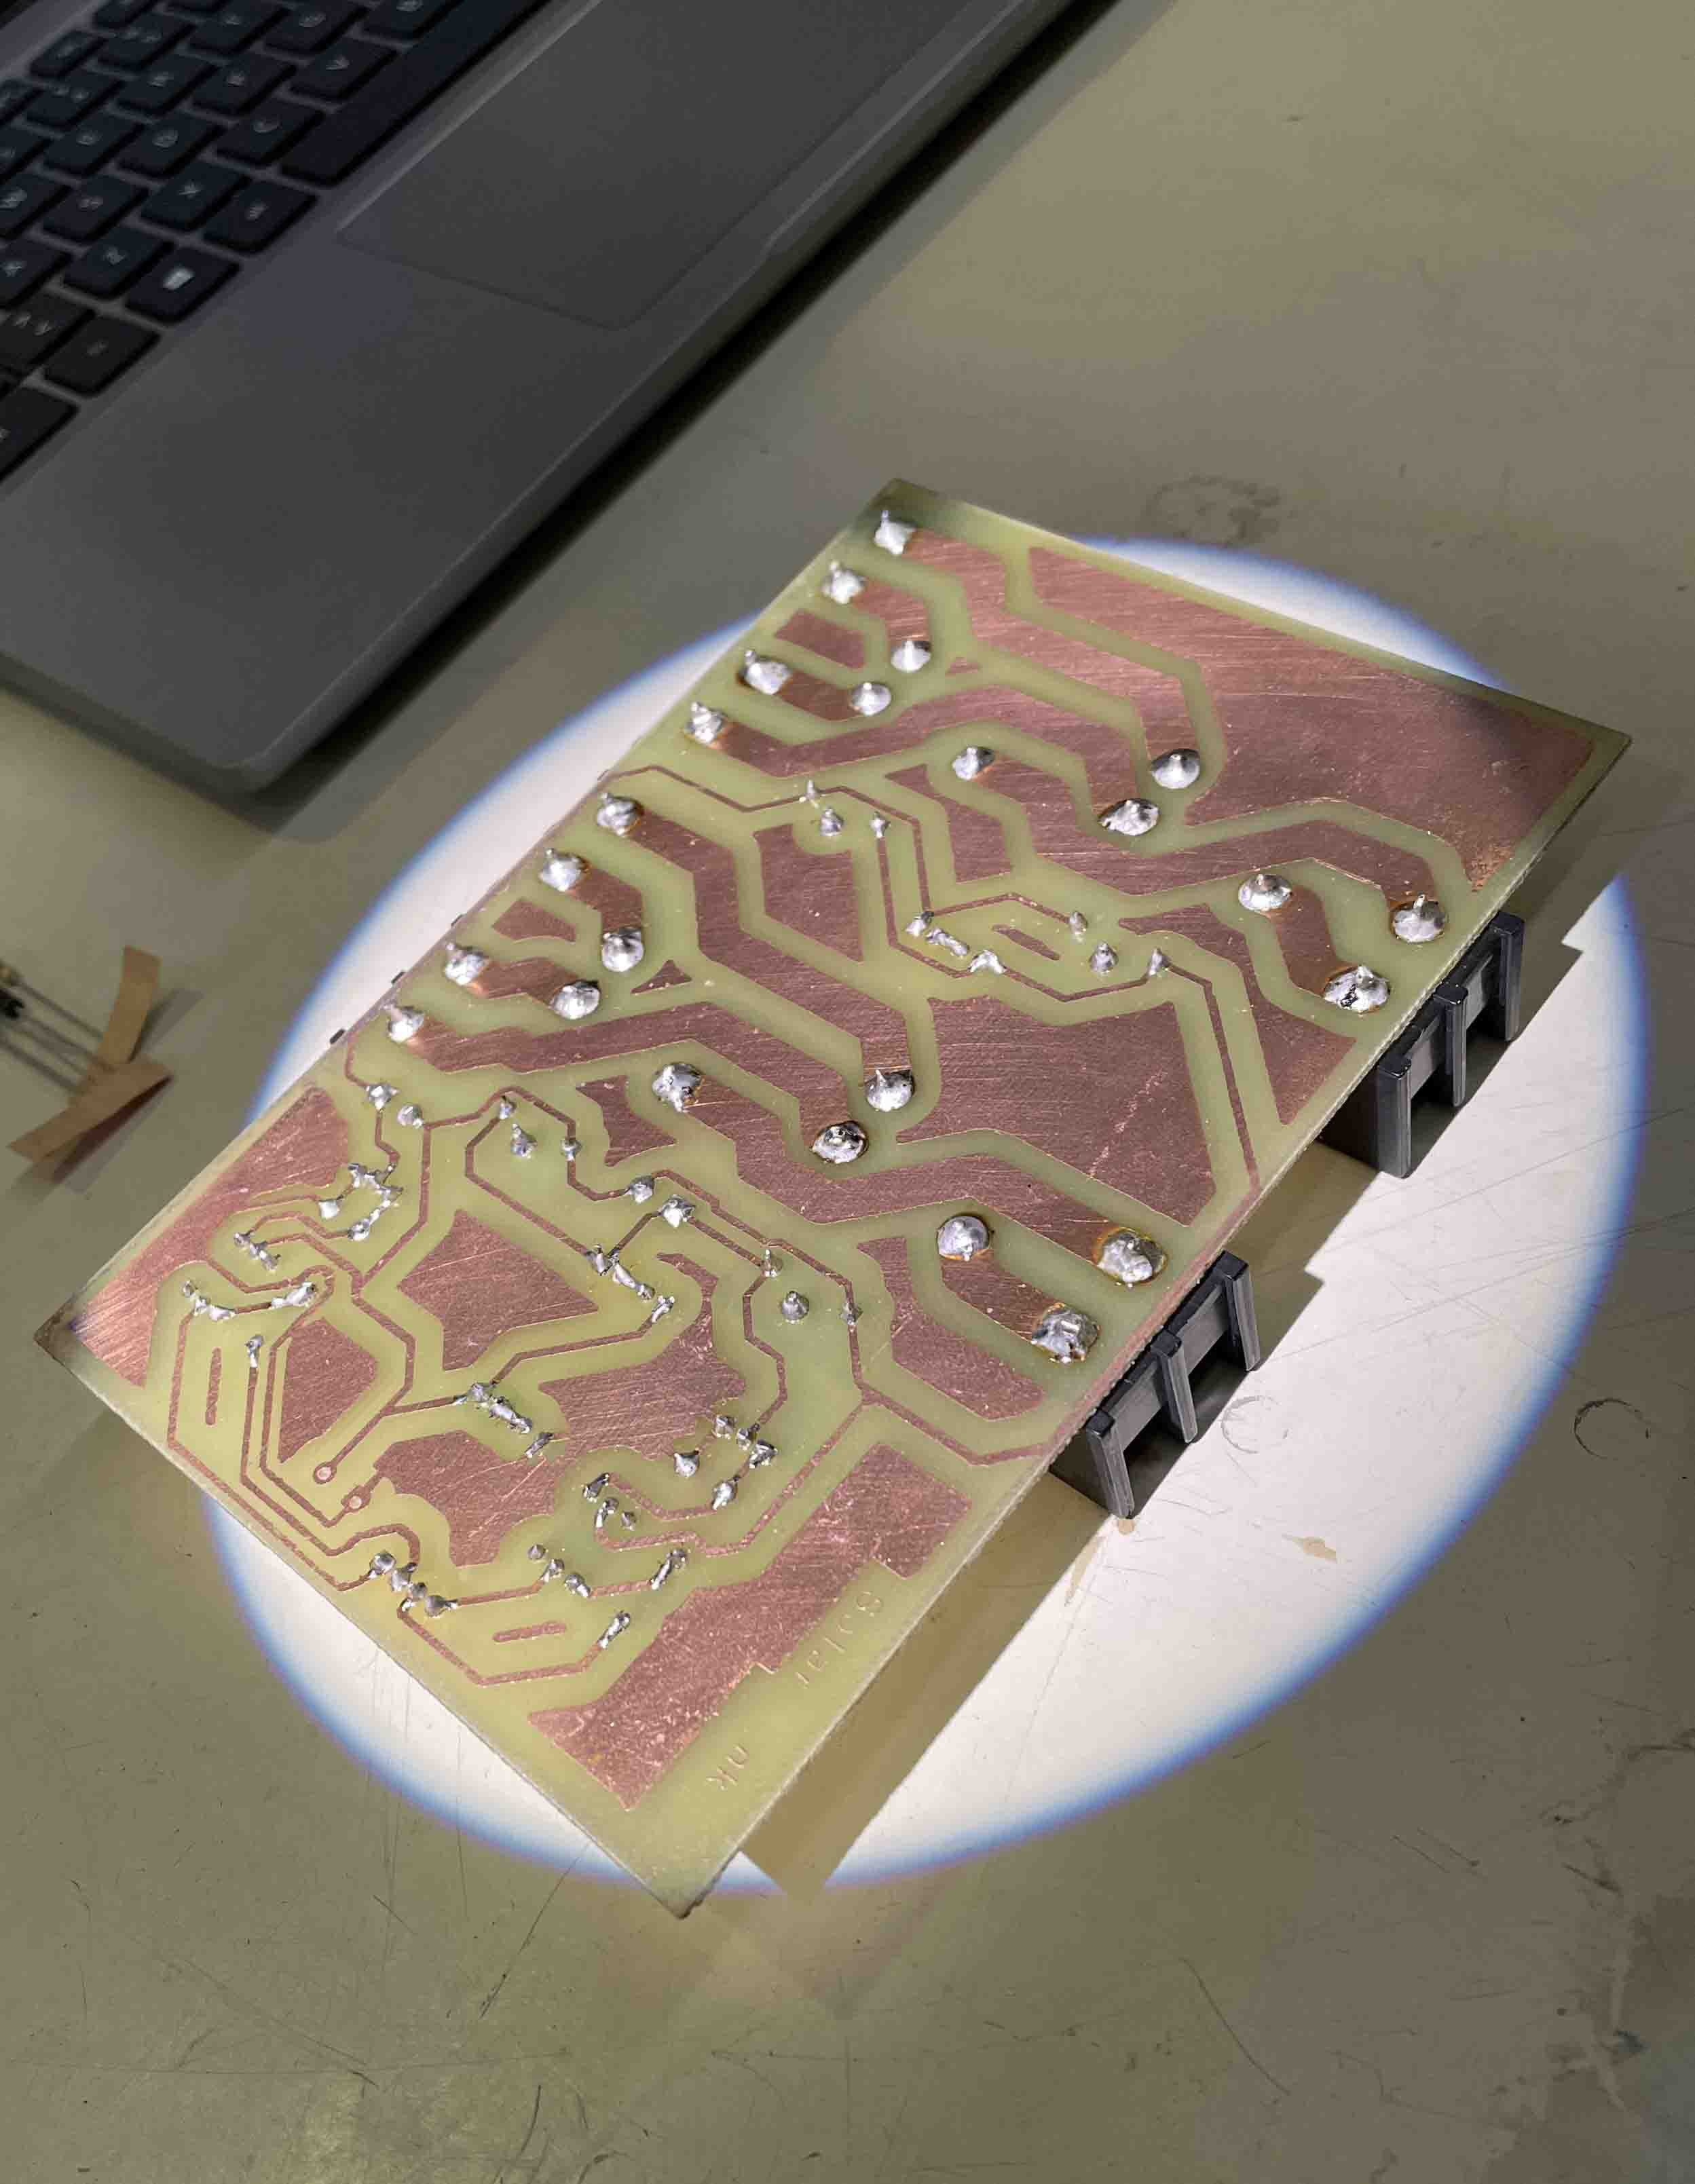
\includegraphics[width=0.9\linewidth]{hardware/IMG_8221.jpg}
\caption{PCB final de conmutación por debajo.}
\label{fig:conm-inf}
\end{subfigure}

\caption{Resultado final del módulo de conmutación.}
\label{fig:image2}
\end{figure}

Este módulo, si bien funciona como debe a la perfección, para nuestro uso presenta un desperfecto: cuando el relé realiza la comutación, hay un punto muerto donde no hay ningún tipo alimentación. Si bien esto se compensa en parte por el cruce por cero, sigue siendo un desperfecto con el cual debemos lidiar.

\subsection{Diseño 3D}
Para presentar el prototipo final en el tablero, fue necesario diseñar una carcasa 3D para cada plaqueta, de tal manera que puedan ser colocadas en un riel DIN y queden protegidas. Cada carcasa fue diseñada especialmente para cada plaqueta, con orificios en los laterales para poder realizar las conexiones, y dejando la parte superior abierta para colocar un acrílico que permita verlas en funcionamiento.\\

\begin{figure}[H]
    \centering
    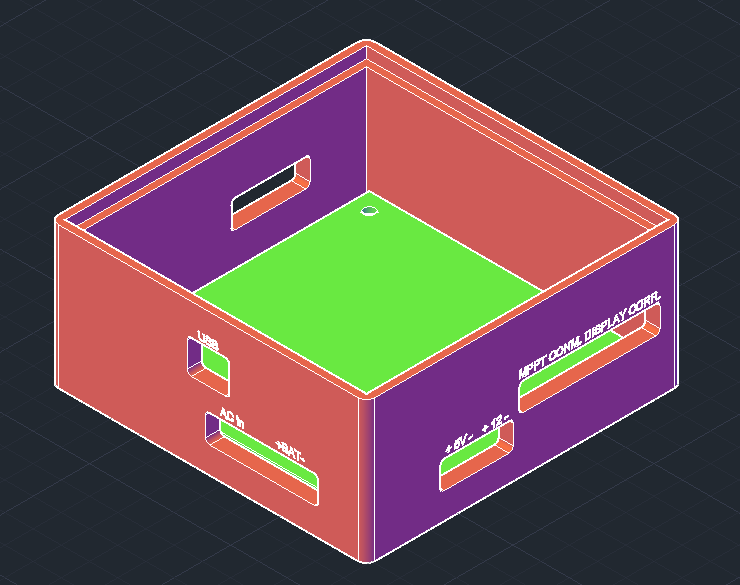
\includegraphics[width=0.75\linewidth]{hardware/Screenshot_22.png}
    \caption{Carcasa 3D para la motherboard.}
    \label{fig:mother-3d}
\end{figure}

\begin{figure}[H]
    \centering
    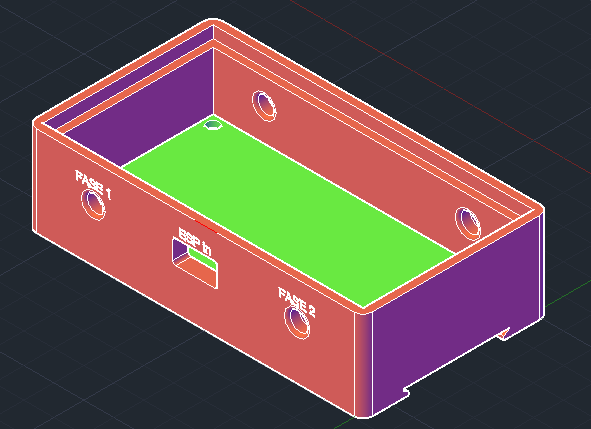
\includegraphics[width=0.75\linewidth]{hardware/Screenshot_21.png}
    \caption{Carcasa 3D para el módulo de medición de corriente.}
    \label{corriente-3d}
\end{figure}

\begin{figure}[H]
    \centering
    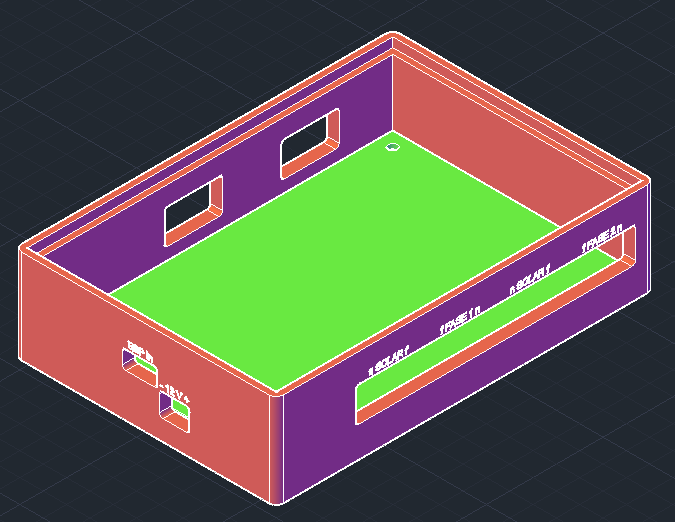
\includegraphics[width=0.75\linewidth]{hardware/Screenshot_20.png}
    \caption{Carcasa 3D para el módulo de conmutación.}
    \label{fig:conmutacion-3d}
\end{figure}

\subsection{Disposición final}

Para armar el tablero, se diseñó una disposición donde la electrónica mas delicada que utilizamos (sobre todo el microcontrolador) quede lo más alejado y aislado posible de la parte de potencia del tablero (principalmente el módulo de conmutación).\\ 

Para lograr la máxima prolijidad posible se utilizaron borneras Zoloda y pasacables, de esta manera se logra que haya muy pocos cables a la vista, y si los hay, es por tramos cortos.\\

\begin{figure}[H]
    \centering
    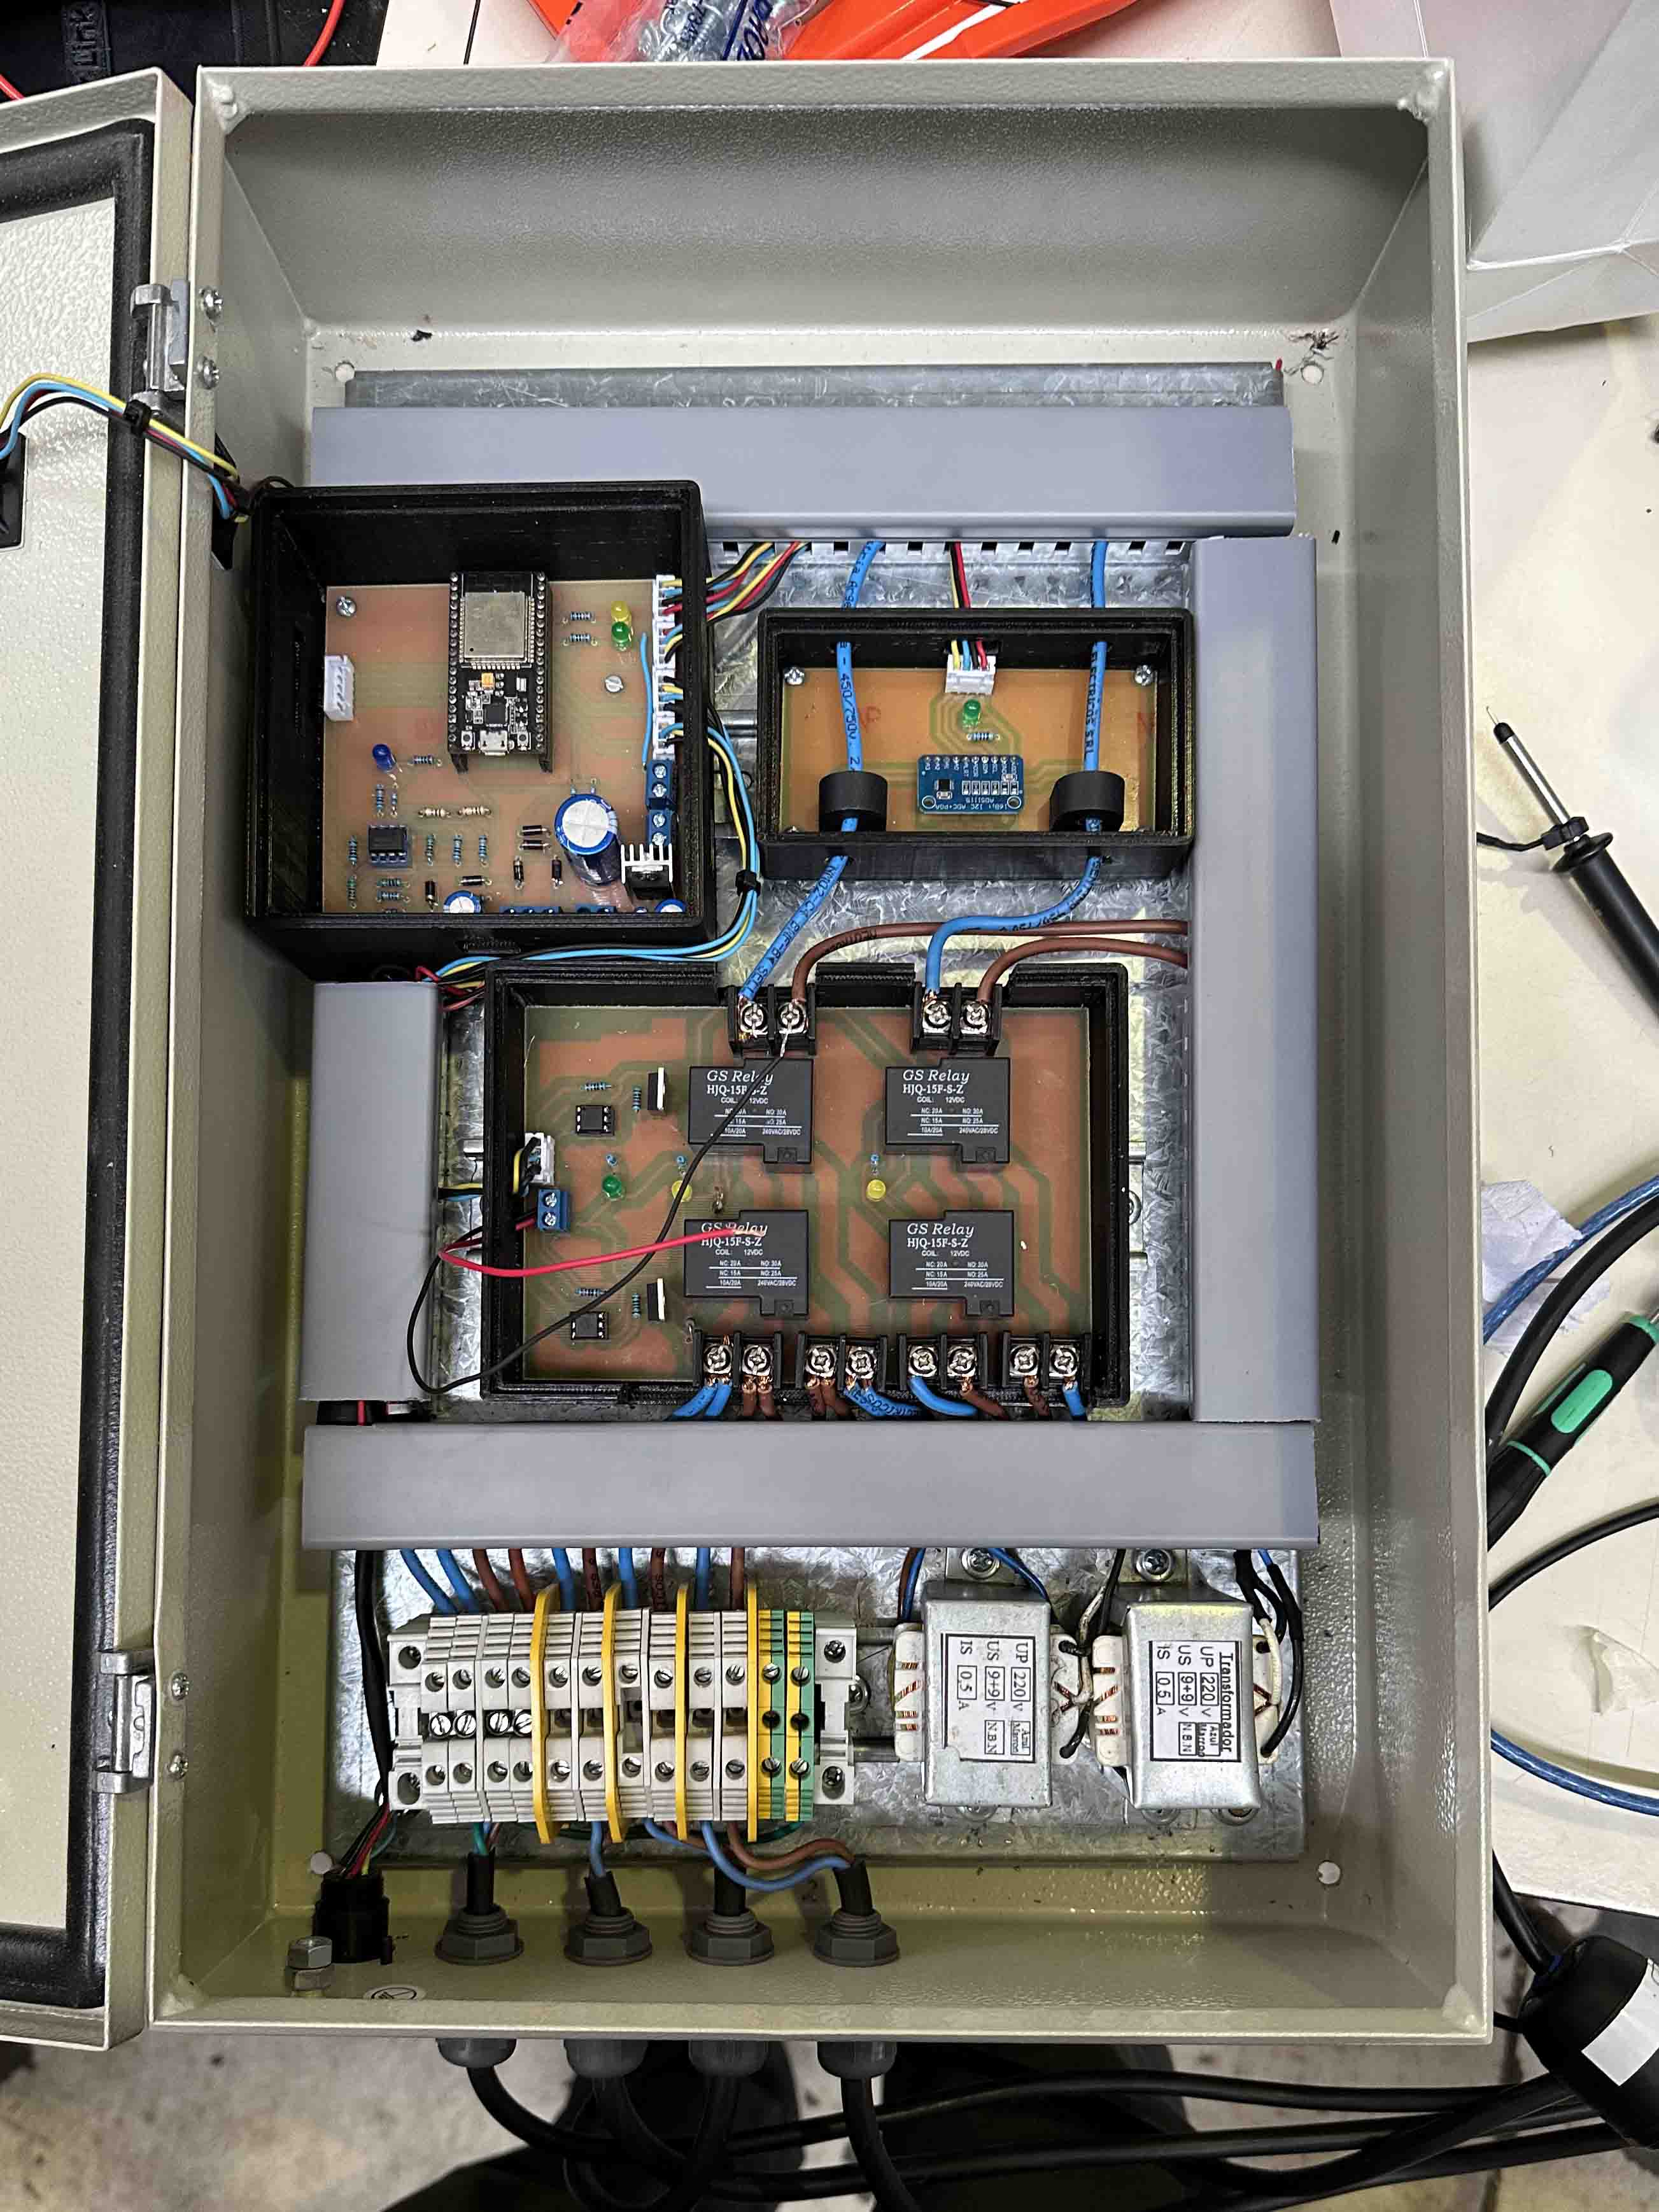
\includegraphics[width=1\linewidth]{hardware/IMG_9354.jpg}
    \caption{Tablero Solar Link.}
    \label{fig:enter-label}
\end{figure}

\begin{figure}[H]
    \centering
    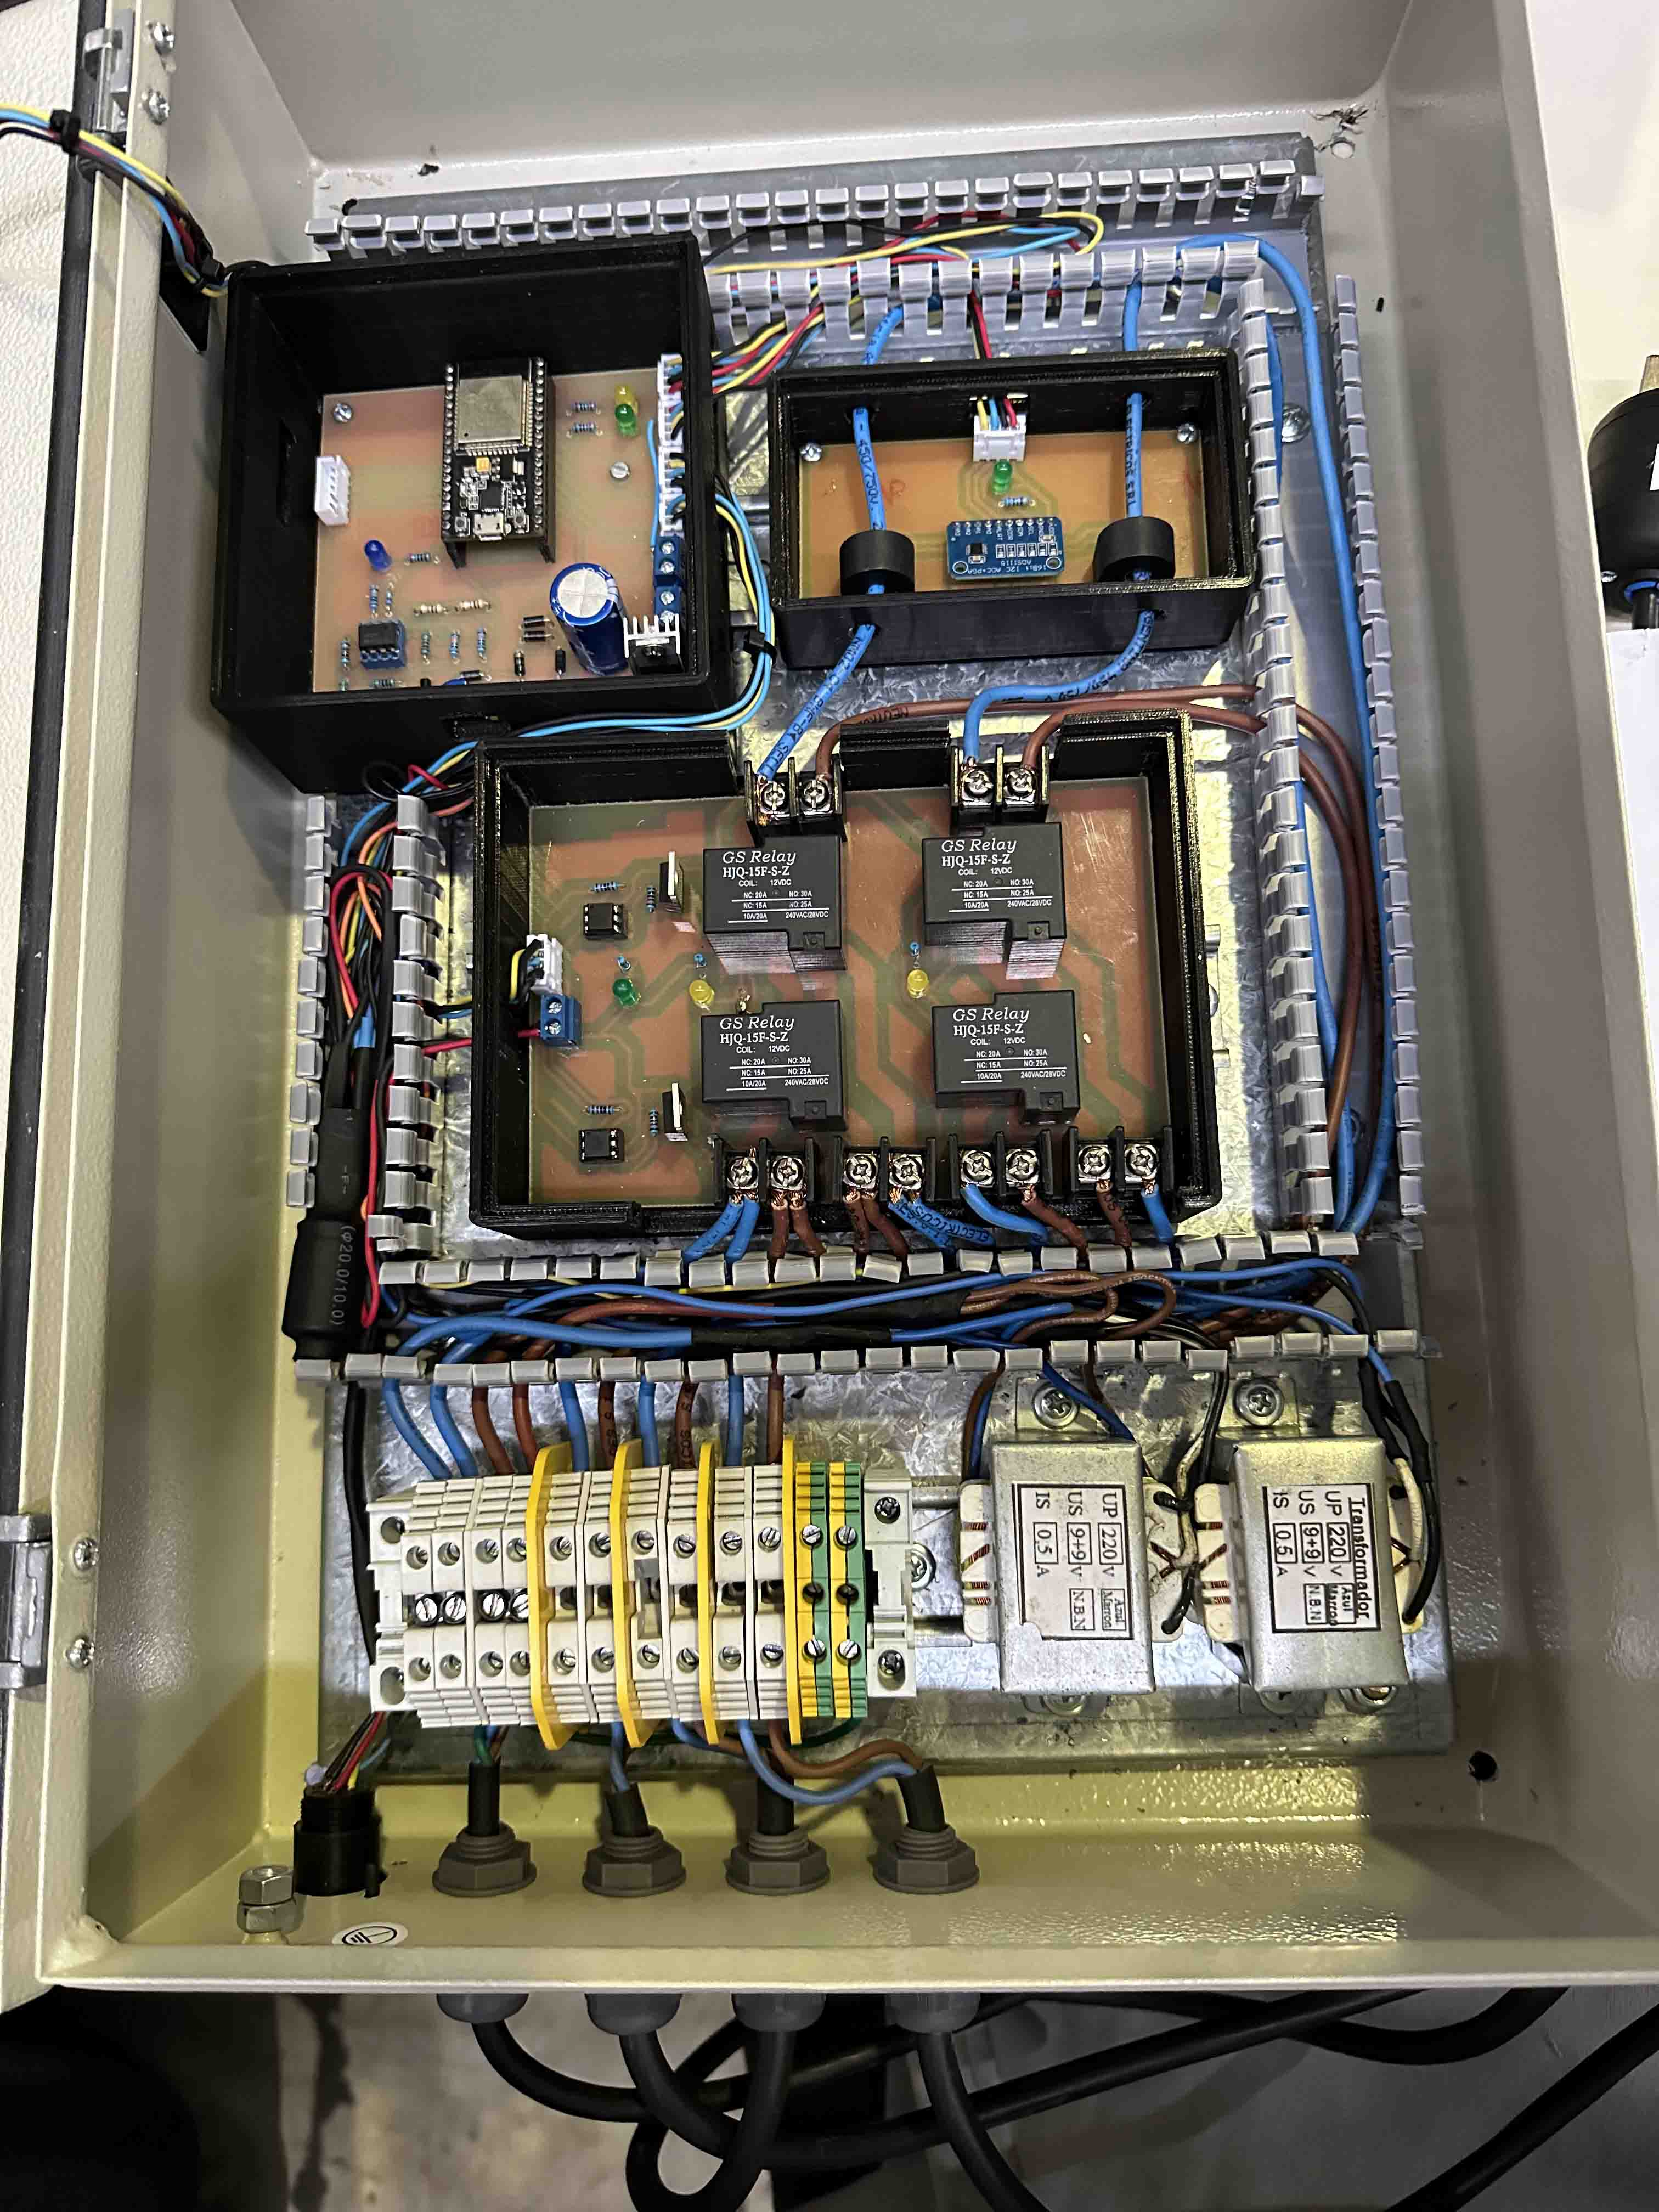
\includegraphics[width=1\linewidth]{hardware/IMG_9352.jpg}
    \caption{Tablero Solar Link con los cablecanales destapados.}
    \label{fig:enter-label}
\end{figure}

